% Options for packages loaded elsewhere
\PassOptionsToPackage{unicode}{hyperref}
\PassOptionsToPackage{hyphens}{url}
%
\documentclass[
]{article}
\usepackage{amsmath,amssymb}
\usepackage{lmodern}
\usepackage{iftex}
\ifPDFTeX
  \usepackage[T1]{fontenc}
  \usepackage[utf8]{inputenc}
  \usepackage{textcomp} % provide euro and other symbols
\else % if luatex or xetex
  \usepackage{unicode-math}
  \defaultfontfeatures{Scale=MatchLowercase}
  \defaultfontfeatures[\rmfamily]{Ligatures=TeX,Scale=1}
\fi
% Use upquote if available, for straight quotes in verbatim environments
\IfFileExists{upquote.sty}{\usepackage{upquote}}{}
\IfFileExists{microtype.sty}{% use microtype if available
  \usepackage[]{microtype}
  \UseMicrotypeSet[protrusion]{basicmath} % disable protrusion for tt fonts
}{}
\makeatletter
\@ifundefined{KOMAClassName}{% if non-KOMA class
  \IfFileExists{parskip.sty}{%
    \usepackage{parskip}
  }{% else
    \setlength{\parindent}{0pt}
    \setlength{\parskip}{6pt plus 2pt minus 1pt}}
}{% if KOMA class
  \KOMAoptions{parskip=half}}
\makeatother
\usepackage{xcolor}
\usepackage{longtable,booktabs,array}
\usepackage{calc} % for calculating minipage widths
% Correct order of tables after \paragraph or \subparagraph
\usepackage{etoolbox}
\makeatletter
\patchcmd\longtable{\par}{\if@noskipsec\mbox{}\fi\par}{}{}
\makeatother
% Allow footnotes in longtable head/foot
\IfFileExists{footnotehyper.sty}{\usepackage{footnotehyper}}{\usepackage{footnote}}
\makesavenoteenv{longtable}
\usepackage{graphicx}
\makeatletter
\def\maxwidth{\ifdim\Gin@nat@width>\linewidth\linewidth\else\Gin@nat@width\fi}
\def\maxheight{\ifdim\Gin@nat@height>\textheight\textheight\else\Gin@nat@height\fi}
\makeatother
% Scale images if necessary, so that they will not overflow the page
% margins by default, and it is still possible to overwrite the defaults
% using explicit options in \includegraphics[width, height, ...]{}
\setkeys{Gin}{width=\maxwidth,height=\maxheight,keepaspectratio}
% Set default figure placement to htbp
\makeatletter
\def\fps@figure{htbp}
\makeatother
\setlength{\emergencystretch}{3em} % prevent overfull lines
\providecommand{\tightlist}{%
  \setlength{\itemsep}{0pt}\setlength{\parskip}{0pt}}
\setcounter{secnumdepth}{-\maxdimen} % remove section numbering
\ifLuaTeX
  \usepackage{selnolig}  % disable illegal ligatures
\fi
\IfFileExists{bookmark.sty}{\usepackage{bookmark}}{\usepackage{hyperref}}
\IfFileExists{xurl.sty}{\usepackage{xurl}}{} % add URL line breaks if available
\urlstyle{same} % disable monospaced font for URLs
\hypersetup{
  hidelinks,
  pdfcreator={LaTeX via pandoc}}

\author{}
\date{}

\begin{document}

\hypertarget{ux8bbaux6587}{%
\section{论文}\label{ux8bbaux6587}}

\hypertarget{ux7eeaux8bba}{%
\section{绪论}\label{ux7eeaux8bba}}

\hypertarget{ux7814ux7a76ux80ccux666fux4e0eux610fux4e49}{%
\subsection{研究背景与意义}\label{ux7814ux7a76ux80ccux666fux4e0eux610fux4e49}}

骨关节炎是一种由遗传因素与环境因素共同作用所产生的关节退行性病变,目前尚无有效的治疗方法。世界范围内至少三亿人罹患骨关节炎且患者群体逐年扩大。而其较差的预后也使得骨关节炎成为了全球范围内导致残疾与疼痛的主要因素之一。临床研究显示,早期诊断与介入对骨关节炎患者病程控制有着积极的影响。因此,构建骨关节炎患病风险预测模型有助于通过早期筛查与预警的方式帮助潜在患者控制病程发展。目前已有诸多关于骨关节炎基因型的全基因组关联研究(GWAS)鉴定了若干骨关节炎的易感SNP位点,也有相关研究基于这些位点建立了骨关节炎风险预测模型。但是这些模型的预测效果较差,远不能达到临床预测的要求。此外,现有的模型也无法处理输入基因型数据之间的复杂网络关系。同时这些模型只能根据输入的位点信息给出判断,无法解释输入位点之间的关联与特定位点在预测过程中的贡献值,模型可解释性方面存在较大不足。以上存在的问题与不足极大限制了骨关节炎风险预测模型的实际应用,如何改进构建模型的方法以提高模型的预测效果,也成为相关研究亟待解决的关键问题。

图作为一种数据结构能通过对节点与边的描述同时反映节点信息与节点之间关系,目前已被广泛应用于分子生物学代谢网络、动物行为学社交网络等生物学领域的研究中。鉴于基因型位点相互关联乃至成网的特征,同时考虑到图在提取和处理处理节点信息(特征)及节点间关系过程中的优势,本文使用图来描述基因型位点特征与位点-位点关系。但是,图数据作为一种非欧数据,传统的诸如卷积神经网络在内的机器学习方法并不适用于直接对图数据进行处理和分析。近年来随着图数据在各个领域的广泛应用,为了解决这一问题,适用于处理图数据的图神经网络因运而生。图神经网络能够基于图信息完成诸如图分类、节点分类等任务并且具有效果好、可解释性强等优点,适合用来处理基因型数据网络。因此,本文将基于图形式的基因型位点,通过图神经网络,结合患者表型信息来构建一种高效的、可解释的骨关节炎风险预测模型。该模型能够基于患者基因型及表型信息,在给出高效患病风险预测结果的同时对患者基因型网络进行解释,因此对骨关节炎的早期诊断与分型具有重要的临床意义。

\hypertarget{ux73b0ux72b6ux7814ux7a76ux7efcux8ff0}{%
\subsection{现状研究综述}\label{ux73b0ux72b6ux7814ux7a76ux7efcux8ff0}}

\hypertarget{ux9aa8ux5173ux8282ux708eux4e0eux98ceux9669ux9884ux6d4bux6a21ux578b}{%
\subsubsection{骨关节炎与风险预测模型}\label{ux9aa8ux5173ux8282ux708eux4e0eux98ceux9669ux9884ux6d4bux6a21ux578b}}

骨关节炎是最常见的关节退行性病变之一,目前报道的案例显示骨关节炎主要影响着人体膝、髋、手等若干关节。骨关节炎的症状主要包括关节疼痛,僵硬、柔韧性丧失,甚至导致关节失能。更严重的是,目前对骨关节炎的治疗以缓解患者痛苦为主,尚无对骨关节的有效临床治愈手段。以上原因也使得骨关节炎成为了导致失能与残疾的主要因素之一,并且严重影响到了患者的生活质量。{[}1{]}同时,骨关节炎在世界范围内有着较庞大的患者群体:世界范围内至少有三亿人罹患骨关节炎{[}2{]},仅在英国范围内的70岁以上群体中就有约40\%的个体受骨关节炎影响{[}3{]},而在全年龄个体中则至少有一千万患者,这导致了每年至少148亿英镑的直接医疗支出{[}4{]}。而研究显示,对骨关节炎的早期诊断与介入能很大程度上延缓关节异常生长进程,对骨关节炎患者的预后改善有着积极的效果{[}1{]}。因此许多研究也将注意力转到了基于风险预测模型的骨关节炎的早期诊断与预防上,目前已有的风险预测模型主要着眼于揭示与骨关节炎病程发展相关的影响因子,包括肥胖,关节错位,关节损伤,骨质增生与高强度的运动{[}6{]}
{[}7{]} {[}8{]}。同时有研究发现骨关节炎也受遗传因素调控。{[}9{]}
并试图通过全基因组关联分析研究骨关节炎的基因背景,以此鉴定并得到了丰富的具有统计学意义、能够作为疾病风险预测模型标志物的疾病易感单核苷酸多态性位点(Single
Nucleotide Polymorphism,SNP){[}10{]}
{[}11{]}。然而,基于这些疾病易感位点建立的风险预测模型性能却不尽如人意:例如Tachmazidou{[}10{]}等人建立的基于PRS算法的风险预测模型,其效果与随机预测相当,远不能达到临床需求,还存在着极大的改进空间。

目前基于基因信息的疾病风险预测模型主要分为两种思路,一种思路通过统计学分析计算个体基因型位点对目标性状的贡献,并根据总体值对样本患病风险进行评估,该方法以PRS为代表{[}12{]}。该方法及其变体已被运用于精神分裂症、I型糖尿病与过敏性肠炎的诊断与筛查中{[}13{]}
{[}14{]}
{[}15{]};另一思路则基于目前具有广泛应用机器学习算法,通过对样本信息进行学习,进而输出模型预测的样本患病风险。构建疾病风险预测模型所常用的机器学习方法主要分为基于回归的机器学习算法与基于树的机器学习算法。前者主要包括决策树与随机森林算法,该算法主要通过构建决策分类规则来完成输入输出数据的建模。有研究便通过随机森林法构建了II型糖尿病的疾病预测模型。{[}21{]}该研究采用的随机森林法相较于基于回归的支持向量机法有着较高的预测准确性。而后者主要有逻辑回归法、支持向量机、神经网络等算法。这类算法通过参数或非参数回归的方法构建损失函数并完成回归计算。这些算法已经被运用于癌症、老年痴呆症、心脏病以及糖尿病的风险预测{[}16{]}
{[}17{]} {[}18{]} {[}19{]}
{[}20{]}。而近年来随着神经网络的广泛应用,基于其发展来的深度学习疾病风险预测模型也受到越来越多的关注。一项研究肥胖预测模型的研究展现了其发掘样本信息的能力
{[}22{]}。相较于传统机器学习算法,深度学习算法具有更好的预测准确性。

但是以上常见的风险预测模型构建方法仍存在着许多问题:首先,对于诸如基因型位点网络或代谢物网络等存在复杂结构的数据,上述方法都无法深层次挖掘数据的内在联系。目前的算法只将输入的位点作为独立的数据点处理,这便会导致输入阶段潜在信息的丧失。其次,这些基于机器学习或者深度学习的方法只能建立从输入数据到输出数据的映射关系,但无法结合输入数据对该映射关系的形成过程给出因果解释,即所谓的``黑箱化''。该问题使得基于以上算法构建的风险预测模型虽然能给出预测值,但是无法因此了解到使得模型做出该预测的决策过程,使得潜藏在输出数据内部的信息被浪费。

综上,目前基于基因型信息的骨关节炎风险预测模型仍存在着预测准确率低,处理网络数据乏力,可解释性差等问题,相关风险预测模型建立的方法亟待改进。

\hypertarget{ux56feux795eux7ecfux7f51ux7edc-1}{%
\subsubsection{图神经网络}\label{ux56feux795eux7ecfux7f51ux7edc-1}}

图是由顶点与边组成的一种数据结构,该数据结构既描述了顶点的性质,也描述了顶点与顶点之间的相关关系。这种数据原理上同生物学领域的许多概念相契合,能够用来描述常见的例如代谢网络、SNP网络的性质。本文主要以图的形式来整合并对输入的SNP数据进行处理。但是,同我们耳熟能详的图片、文本、序列等数据不同,图数据不满足平移不变性,不能投影到欧几里得空间中。而平移不变性又是目前常见的诸如卷积神经网络,递归神经网络等深度学习网络所依赖的关键假设。{[}23{]}
因此这些神经网络不能被直接用来处理图数据。但是随着图数据的广泛应用,能够处理图数据的神经网络也在逐渐发展。A.
Sperduti and A. Starita{[}24{]}
首先提出了一种能够应用于有向无环图的神经网络,这也被认为是图神经网络研究的开端。Gori{[}25{]}等人则正式提出了图神经网络这一概念。而随着卷积方法在传统的成功,图卷积方法也成为了图神经网络中一项热门的研究方向,并产生了诸多已被应用到实际生产生活的神经网络框架。

图卷积神经网络根据卷积核功能分为两种类:基于空间的图卷积与基于谱的图卷积。基于空间的卷积借助了信息传播{[}25{]}的思想,认为图中的节点信息通过边进行扩散,卷积核作用于节点的空间邻域,继而通过该空间邻域计算节点信息。目前得到广泛应用的空间卷积算法主要有GIN{[}26{]},GAT{[}27{]},DCNN{[}28{]}等;而基于谱的图卷积则借助图的拉普拉斯量将图结构于傅里叶空间展开,有助于识别图结构中的潜藏结构。基于这一方法的谱卷积方法主要有GCN{[}29{]},ChebyNet{[}30{]},AGCN{[}31{]}等。目前图神经网络已被广泛应用于包括药物筛选{[}32,33{]},计算机视觉{[}34{]}等图数据的分析。Ghosal{[}35{]}等人便将图神经网络用于阿尔兹海默症疾病风险的基因型预测,证明了使用图神经网络构建基于基因型的疾病风险预测模型的可行性。

此外,由于图的结构及其蕴含的信息特点,也有研究{[}36{]}开发出了对图神经网络的解释器。该解释器通过分析已训练好的图神经网络与预测结果,给出与预测结果相关的子图。利用该类型解释器,我们可以在生成风险预测结果时同时获取与该预测结果相关的子图信息,并为致病位点或疾病分型相关工作提供便利。而这类型工作是传统疾病预测模型所无法实现的。

\hypertarget{ux672cux6587ux7814ux7a76ux5185ux5bb9}{%
\subsection{本文研究内容}\label{ux672cux6587ux7814ux7a76ux5185ux5bb9}}

综上所述,本文将基于谱图卷积网络,试图构建一个可解释的基于患者基因型信息与表型信息的高效骨关节炎风险预测模型。本文工作主要分为三个方面:首先,本文根据目前已发表的GWAS研究及公共数据库UK
BioBank获取患者表型与基因型数据并进行数据预处理;之后构建了包括特征筛选、邻接矩阵估计、图卷积神经网络、表型信息融合四个模块在内的骨关节炎风险预测模型;最后本文对该模型的性能以及预测结果进行了进一步的分析和解读,继而对模型的预测准确性,可解释性等指标进行评估。具体研究内容分为以下五个章节

第一章,绪论。该章首先阐述论文的研究背景与意义,并对骨关节炎、风险预测模型以及图神经网络领域加以综述。最后介绍了本文的主要研究内容。

第二章,数据获取。该章介绍了根据已有研究从公共数据库获取患者基因型与表信息以及根据一定评判标准对该数据进行筛选与预处理的过程。

第三章,风险预测模型搭建。该章介绍了从特征筛选、邻接矩阵估计、图卷积神经网络、表型信息融合四个模块出发构建骨关节炎风险预测模型的过程与理论原理。

第四章,模型性能评价。该章分析了本文搭建模型的预测准确率并将其同传统风险预测模型准确率进行比较。同时还从模型可解释性角度出发分析了模型预测结果。一方面证明本文建立模型相较于传统模型具有较高程度的提升,另一方面也展现了模型对骨关节炎性状之外信息的揭示能力。

第五章,总结与展望。总结本文的研究工作,并对未来的研究方向进行展望。

\hypertarget{ux6570ux636eux83b7ux53d6}{%
\section{数据获取}\label{ux6570ux636eux83b7ux53d6}}

\hypertarget{ux6570ux636eux6765ux6e90}{%
\subsection{数据来源}\label{ux6570ux636eux6765ux6e90}}

本文所使用的基因型与表型数据主要来自于UK
Biobank{[}37{]}数据库。该数据库收集并整合了2006-2010年间于英国招募的约500000名志愿者的生物样本、身体状况、功能评估、多种表型及遗传学数据。由于其所提供的丰富多样的遗传与表型信息,UK
Biobank已经成为了研究多种复杂表型和遗传病的重要数据来源。本文主要基于UK
Biobank的第三批发布数据开展骨关节炎相关研究。

\hypertarget{ux6837ux672cux6807ux6ce8}{%
\subsection{样本标注}\label{ux6837ux672cux6807ux6ce8}}

我们从UK
Biobank数据库中获取骨关节炎患者(阳性样本)与非骨关节炎患者(阴性样本)。UK
Biobank所提供的信息我们使用个体疾病伤害分类标准编码来对样本进行区分。国际疾病伤害及死因分类标准(The
\textbf{I}nternational Statistical \textbf{C}lassification of
\textbf{D}iseases and Related Health
Problems,ICD)是由世界卫生组织所制定的根据特定规则对人群可能出现疾病进行归类的一套编码系统。{[}38{]}
UK
Biobank已经对数据库内样本进行了ICD标注,因此我们可通过这一方法筛选研究对象。

参考其他骨关节炎的相关研究,{[}10{]}我们确定如下筛选规则。我们认定包含如下ICD编码的个体为骨关节炎患者。

\begin{longtable}[]{@{}ll@{}}
\toprule()
ICD编码 & 分类 \\
\midrule()
\endhead
M15-X & 骨关节炎 \\
M16-X & 髋关节炎 \\
M17-X & 膝关节炎 \\
M18-X & 腕掌关节关节炎 \\
M19-X & 其他关节炎 \\
\bottomrule()
\end{longtable}

在筛选非骨关节患者时,为防止其他关节症状的干扰,我们也根据文献报道对包含另一些编码的个体予以排除。

\begin{longtable}[]{@{}ll@{}}
\toprule()
ICD编码 & 分类 \\
\midrule()
\endhead
M11-X & 软骨钙化症 \\
M20-X、M21-X & 获得性关节畸形 \\
M22-X & 髌骨功能异常 \\
M23-X & 膝关节异常 \\
M24-X & 其他关节异常 \\
M25-X & 关节疼痛 \\
M42-X & 脊柱软骨病 \\
\bottomrule()
\end{longtable}

依照以上规则,我们从UK
Biobank数据库中筛选并获得6706名骨关节炎患者作为模型训练的阳性集。同时,为保证风险预测模型训练数据的均衡性,我们又挑选出了7000名正常个体作为阴性集。两部分数据共同构成本次研究所使用的数据集。

\hypertarget{ux57faux56e0ux578bux4f4dux70b9ux9009ux53d6}{%
\subsection{基因型位点选取}\label{ux57faux56e0ux578bux4f4dux70b9ux9009ux53d6}}

人类基因组具有复杂性与多样性,本研究中的每个样本个体基因型数据都由数十万乃至数百万个基因型位点组成。由于目前任何算法都无法短时间内对如此多的样本进行处理,因此需要从其中选取部分具有统计学意义的位点。本文根据目前已发表的骨关节炎的GWAS结果{[}10{]}
{[}11{]}对样本的基因型位点进行关联显著值(P-Value)与等位基因频率(Allele
Frequency,AF)选取。

\hypertarget{ux663eux8457ux503c}{%
\subsubsection{显著值}\label{ux663eux8457ux503c}}

关联显著值是用来衡量GWAS研究中单核苷酸突变与给定性状关联显著性的一个统计量。在GWAS研究中,我们设定零假设为数据中没有SNP位点与特定性状相关联;而备择假设为至少有一个SNP位点同特定性状相关联。同时我们定义统计量\(p\)为当零假设为真时观察到该关联的概率。显然,\(p\)值越小,有越高把握在观察到关联时认为零假设为假。因此我们可以设定一个阈值,当统计量\(p\)低于该阈值时拒绝原假设,认为该位点同目标性状相关。{[}39{]}

但是,由于遗传漂变的影响,随机的基因突变也有可能具有类似相关关系。因此我们并不能认为\(p\)值较小的位点同目标位点直接相关,在指定阈值时需要将可能由遗传漂变所产生的位点筛去。因此我们还需要通过QQ图来完成阈值界定。QQ图是一种根据分位数对两概率分布所作的图,该图来比较两分布差别的方式。{[}40{]}
GWAS中的QQ图横轴为遗传漂变所产生的分布,纵轴为实际分布,当图像偏离对角线时认为这类数据并非随机漂变。因此,根据QQ图本文确定p阈值为\(10^{-5}\)。

\hypertarget{ux7b49ux4f4dux9891ux7387}{%
\subsubsection{等位频率}\label{ux7b49ux4f4dux9891ux7387}}

在GWAS研究中往往会发现一些出现频率很低的突变。受限于GWAS原理,大多数研究不能很好计算低等位频率位点与性状的相关性。因此在实际研究时,还需要通过等位基因频率对所得位点进行进一步筛选。根据文献我们将该阈值设定为0.05{[}41{]}。

综上,本文根据关联分析显著值与等位基因频率对所得SNP位点进行筛选,最终每个个体选取选取8687个SNP位点作为待分类基因型位点。同时,我们根据位点目标突变的出现频率对数据进行编码,将基因型信息转化为算法可直接读取的数值信息。

\hypertarget{ux7279ux5f81ux7b5bux9009}{%
\subsection{特征筛选}\label{ux7279ux5f81ux7b5bux9009}}

目前我们已经从UKB数据库中选取了6706位骨关节炎患者作为阳性样本,每个患者包括8687个基因型特征。考虑到特征数大于样本数,可能对预测模型的准确率产生不利影响。{[}42{]}本文还使用卡方法与支持向量机法对现有数据进行了特征筛选。

\hypertarget{ux57faux4e8eux5361ux65b9ux7684ux7279ux5f81ux7b5bux9009}{%
\subsubsection{基于卡方的特征筛选}\label{ux57faux4e8eux5361ux65b9ux7684ux7279ux5f81ux7b5bux9009}}

卡方法使用统计学方法对输入特征与样本标注的关联进行计算,并根据计算结果筛选与样本标注相关程度较高的特征。其具体过程如下:

\begin{enumerate}
\def\labelenumi{\arabic{enumi}.}
\item
  确定零假设与备择假设:对于特征与样本标注
  ,定义零假设\(H_0\)为该特征与样本标注无关;定义备择假设\(H_1\)为该特征与样本特征相关
\item
  计算特征卡方值:根据公式计算特征与样本标注的卡方值

  \[\chi_c^2=\sum \frac{(O_{i}-E_i)^2}{E_i}\]

  其中:

  \begin{itemize}
  \item
    \(c\) 为该卡方分布的自由度
  \item
    \(O\) 为观测值
  \item
    \(E\) 为期望值
  \end{itemize}
\item
  查卡方表,拒绝或接受假设:对于计算所得卡方值,查卡方表。对照计算所得卡方值与一定自由度与置信度下的标准卡方值。当计算卡方值大于标准卡方值时接受零假设,认为该特征与样本标注无关;当计算卡方值小于标准卡方值时拒绝零假设,认为该特征与样本标注相关。基于此选择该特征
\end{enumerate}

\hypertarget{ux57faux4e8eux652fux6301ux5411ux91cfux673aux7684ux7279ux5f81ux7b5bux9009}{%
\subsubsection{基于支持向量机的特征筛选}\label{ux57faux4e8eux652fux6301ux5411ux91cfux673aux7684ux7279ux5f81ux7b5bux9009}}

支持向量机(Support Vector
Machine)是一种著名的机器学习算法。其通过构建数据空间内的分类平面来实现数据分类算法。其算法核心为以下优化过程

\[\min_{W,b} [C\sum_{i}max(0,1-y_i(X_i^TW+b))+l(W)]\]

其中:

\begin{itemize}
\item
  \(X_i\) 为样本数据
\item
  \(W,b\)为超平面参数
\item
  \(y_i\)为样本标注
\item
  \(C\)为惩罚系数,即错误分类情况下对优化函数的惩罚
\item
  \(l(W)\)为超平面拟合程度的评价函数
\end{itemize}

从上式可以看出,该优化目标主要分为两部分:一部分衡量超平面对数据点的分类能力;另一部分衡量超平面对数据的拟合能力。目前常用的SVM算法中

\[l(W)=\frac{1}{2}w^Tw\]

此时该拟合函数评价分离两类数据点超平面在超空间上的距离。距离越大,证明该超平面对数据的拟合能力越好。但是,当该函数变为

\[l(W)=e^T|w|\]

此时该拟合函数又称\(w\)的 \(l_1\)
范数,又称Lasso惩罚{[}43{]},该范数可以用来评价特征在整体分类效果中的贡献{[}44{]}。因此本文可通过该范数对特征进行筛选。

\hypertarget{ux672cux7ae0ux5c0fux7ed3-1}{%
\subsection{本章小结}\label{ux672cux7ae0ux5c0fux7ed3-1}}

本章介绍了本文所使用数据集获取与预处理过程。首先,根据ICD编码我们从UKB数据库中筛选并获得了6706名患病个体(阳性集)与7000名非骨关节炎个体(阴性集)作为研究对象。其次,根据关联分析显著性及基因频率从已发表的骨关节炎GWAS中筛选出感兴趣的位点并获取研究样本相应的基因型数据,之后再根据位点信息对其进行编码。最后,为了进一步减少无关的样本特征,加快计算速度,本文通过卡方法与支持向量机法对数据进行特征筛选。最终完成了骨关节炎风险预测模型基因型数据集的构建。

\hypertarget{ux9aa8ux5173ux8282ux708eux98ceux9669ux9884ux6d4bux6a21ux578bux6784ux5efa}{%
\section{骨关节炎风险预测模型构建}\label{ux9aa8ux5173ux8282ux708eux98ceux9669ux9884ux6d4bux6a21ux578bux6784ux5efa}}

第二章我们获取了骨关节炎患者的基因型数据并对其进行了预处理与特征筛选。本章则主要对骨关节炎风险预测模型做以介绍。该模型首先根据基于变分期望最大化算法的图估计器构建了输入基因型数据的关联并通过图来表示该关联关系。之后构建了图神经网络对建立的图进行学习与处理。该模型还通过融合患者表型进一步增强模型性能。最后本模型还构建了基于预测值与输入数据的模型解释器。

\hypertarget{ux56feux4f30ux8ba1ux5668}{%
\subsection{图估计器}\label{ux56feux4f30ux8ba1ux5668}}

\hypertarget{ux56feux795eux7ecfux7f51ux7edcux4e2dux65e0ux7ed3ux6784ux6570ux636eux7684ux5904ux7406ux65b9ux6cd5}{%
\subsubsection{图神经网络中无结构数据的处理方法}\label{ux56feux795eux7ecfux7f51ux7edcux4e2dux65e0ux7ed3ux6784ux6570ux636eux7684ux5904ux7406ux65b9ux6cd5}}

图神经网络只适用于图类型的数据,对常见无结构数据(例如文本,图像)的处理较为困难。本文目前获得的基因型数据也属于无结构数据,原理上不适用于图神经网络。但是,考虑到图神经网络优秀的性能与可解释性,我们需要基于该无结构基因型数据构建图,继而输入图神经网络。目前根据无结构数据建图的方法主要有两种方法:一种是通过分析数据构建静态图,神经网络训练过程中不对该图结构加以更新{[}45{]}
{[}46{]},例如在处理无结构的图像数据时,Monti{[}46{]}提出了一种通过超像素将图像数据转为图的方法,使得图神经网络能够处理图像数据;第二种是通过学习方法构建动态图结构,并在网络训练过程中不断更新图结构{[}47{]}。这类通过学习方法获取图结构特征的过程也被称为图结构学习(Graph
Structure
Learning,GSL)。目前的图结构学习过程主要分为三个步骤:首先通过已知数据通过k近邻法{[}48{]}或者阈值法{[}49{]}构建出一个初始图结构或观测图结构;然后使用诸如随机块模型(Stochastic
Block
Model,SBM){[}50{]}对该观测图结构进行建模;最后通过算法估计出数据可能具有的图结构。在图估计的过程中,基于统计学的算法受到了广泛关注:例如Zhang{[}51{]}等人提出了一种基于贝叶斯思想的图估计器。其认为图结构根据依赖一定参数的分布所产生,如果通过蒙特卡洛方法对该参数进行估计,就可因此得到该分布的具体信息,继而对图结构进行估计。Elinas{[}52{]}同样基于贝叶斯思想提出了一种使用变分推断法的图估计方法。这类贝叶斯方法思路简洁,原理清晰。因此,本文也将基于贝叶斯思想构建图结构估计器。

\hypertarget{ux95eeux9898ux63cfux8ff0}{%
\subsubsection{问题描述}\label{ux95eeux9898ux63cfux8ff0}}

贝叶斯思想认为:事件的观测值并不能反映事件的真实特性。贝叶斯方法因此主要解决由事件观测值向事件真实值的推断过程。但是在讨论推断过程前,我们首先需要对观测值与真实值加以定义。

\hypertarget{ux89c2ux6d4bux503cux6784ux5efa}{%
\paragraph{观测值构建}\label{ux89c2ux6d4bux503cux6784ux5efa}}

对于本文研究对象基因型数据而言,未经图神经网络处理的原始数据所含信息量较少,较难依据初始数据构建观测值。但是有研究显示,经过谱图神经网络处理之后,具有较强关联的节点具有相似的值。{[}53{]}
我们因此认为在图神经网络的输出值中,对任一节点,如果有一其他节点与其有着相似的值,则两节点之间可能存在关联。
这种关联可以通过k近邻算法{[}48{]}计算从而得到k近邻网络,而该k近邻网络可以很好地描述节点的局部特征。在Wang{[}54{]}等人的研究中,也有通过根据图神经网络输出值构建k近邻网络的描述。我们因此根据每个样本经图神经网络处理后的输出值建立k近邻网络,再将所有网络相加求平均以获得单个观测值。同时为了防止信息丢失,我们将首次经图神经网络处理时输入的图初始化为全连接图,即认为每个节点都同其他节点存在关联。

\hypertarget{ux771fux5b9eux503cux6784ux5efa}{%
\paragraph{真实值构建}\label{ux771fux5b9eux503cux6784ux5efa}}

本研究中所感兴趣的真实值为实际的未知图结构。但是对图结构的直接计算过于复杂,我们因此需要将图结构参数化,即使用少数几个参数来描述图结构。目前在图论领域常用的图参数化模型为随机块模型{[}50{]},该模型认为图中的节点属于某几个簇,节点之间是否相连仅与两节点所在的簇相关且服从某一参数化分布。因此我们只需要得出支配该分布的参数就能对图结构加以复现,继而用少数参数描述庞大的网络。因此本文将该类参数作为推断的目标,而由其产生的图结构作为模型输出值。

\hypertarget{ux63a8ux65adux8fc7ux7a0b}{%
\paragraph{推断过程}\label{ux63a8ux65adux8fc7ux7a0b}}

界定了观测值与真实值之后,我们便可对图估计器所解决的问题加以严谨描述。

图估计器首先根据图神经网络的输出构建观测值\( O\) ,其中

\[O^{ij}=\frac{1}{N}\sum_N o^{ij}_n\]

\(O^{ij}\)描述了节点\(i,j\)之间关联的观测值,\(N\)为样本数,\(o^{ij}_n\)为由第\(n\)个样本神经网络输出值构建的k近邻网络中节点\(i,j\)之间的关联。通过该观测值我们构建图
\(G=(V,O)\),其中\(V=\{v_1,...v_n\}\)描述图中节点,即样本基因型位点。

为了通过SBM模型参数化图结构,我们假定图中共含有\(C\)个簇,每个节点\(i\)从属于簇\(m\)的概率用
\(z_{im}\in \bold{Z}^{N\times C},i\in \{1, ... ,n\},m\in\{1,...,C\}\)来描述,且\(z_i\)相互独立并满足多项分布

\[z_i ~^{iid} M(1,\alpha)\]

基于此,我们使用\(z_i\)
来描述节点之间关联。我们认为任意两节点之间的关联相互独立并满足二项分布

\[o_{ij}|z_{im},z_jn = 1 ~ B(1,\pi_{z_iz_j})\]

可以看出,只要解出参数\(\pi\)与\(\alpha\),就可以此构建出一个SBM模型,继而对图结构加以推断;因此本文给出以下目标:

\begin{quote}
基于观察到的节点关联信息\(O\)以及隐变量\(Z\),估计参数\(\theta=\{\alpha,\pi\}\),并根据该参数给出推断图结构

\[\hat{\theta}=argmax l_\theta(O)\]
\end{quote}

\hypertarget{ux57faux4e8eux53d8ux5206ux671fux671bux6700ux5927ux5316ux7684ux56feux4f30ux8ba1}{%
\subsubsection{基于变分期望最大化的图估计}\label{ux57faux4e8eux53d8ux5206ux671fux671bux6700ux5927ux5316ux7684ux56feux4f30ux8ba1}}

\hypertarget{ux63a8ux5bfcux4e0eux6574ux7406}{%
\paragraph{推导与整理}\label{ux63a8ux5bfcux4e0eux6574ux7406}}

在节点关联与节点簇信息均已知的情况下,我们首先计算似然函数\(l_{\theta}\),根据边缘概率公式,有

\[l_\theta(O)=\sum_{Z}\log p_\theta(O,Z)=\sum_Z(\log p_{\pi}(O|Z)
+\log p_\alpha(Z))\]

其中

\[\sum_Z(\log p_{\pi}(O|Z)+\log p_\alpha(Z))=\sum_Z(\sum_{i,j}^{n}\sum_{m,n}^C\log p_\pi(o_{ij}|z_{im}z_{jn})
+\sum_{i}^N\sum_m^C\log p_\alpha(z_{im}))\]

给定参数时,有

\[p_\pi(o_{ij}|z_{im}z_{jn};\pi)=\binom{1}{O_{ij}}[\pi_{mn}(1-\pi_{mn})^{1-O_{ij}}]^{ z_{im}z_{jn}}\]

\[p_\alpha(z_{im})=\alpha_m^{z_{im}}\]

可得

\[l_\theta(O;\theta) = \sum_Z(\sum_{i,j}^{n}\sum_{m,n}^C\log p_\pi(o_{ij}|z_{im}z_{jn})+\sum_{i}^N\sum_m^C\log p_\alpha(z_
{im}))\\ =\sum_Z(\sum_{i,j}^{n}\sum_{m,n}^C\log \binom{1}{O_{ij}}[\pi_{mn}(1-\pi_{mn})^{1-O_{ij}}]^{ z_{im}z_{jn}}+\sum_
{i}^N\sum_m^C\log\alpha_m^{z_{im}})\]

\hypertarget{ux671fux671bux6700ux5927ux5316ux7b97ux6cd5}{%
\paragraph{期望最大化算法}\label{ux671fux671bux6700ux5927ux5316ux7b97ux6cd5}}

考虑到似然函数中含隐变量\(Z\),通常我们采用期望最大化算法{[}55{]}计算使得似然函数取极大的参数。我们对似然函数做如下处理

\[l(O;\theta)=\log p(O;\theta)\\
=\log \int_Zp(O,Z;\theta)dz\\
=\log \int_Z q(Z)\frac{p(O,Z;\theta)}{q(Z)}dz\\
=\log \mathop{\mathbb{E}}[\frac{p(O,Z;\theta)}{q(Z)}]\]

其中\(q(Z)\)为一辅助函数且满足\(\int q(Z)=1\)。根据Jensen不等式{[}58{]},对任意一凸函数,有

\[\mathop{\mathbb{E}}[f(x)]\leq f(\mathop{\mathbb{E}}[x])\]

当且仅当\(x=\mathop{\mathbb{E}}[x]\)时等号成立。又因为\(\log x\)
为一凸函数,因此有

\[l(O;\theta)=\log p(O;\theta)\\
=\log \mathop{\mathbb{E}}[\frac{p(O,Z;\theta)}{q(Z)}]\\
\geq  \mathop{\mathbb{E}}[\log\frac{p(O,Z;\theta)}{q(Z)}]\]

当且仅当

\[\frac{p(O,Z;\theta)}{q(Z)}=c\]

时取等(\(c\)为一常数)。对该式进行变化,有

\[q(Z)=c\cdot p(O,Z;\theta)\]

又因为\(\int q(Z)dz=1\),有

\[\int_Z q(Z)dz=\int_Z c\cdot p(O,Z;\theta)dz=1\\
c=\frac{1}{\int_Zp(O,Z;\theta)dz}\]

因此

\[q(Z)=\frac{p(O,Z;\theta)}{\int_Zp(O,Z;\theta)dz}=\frac{p(O,Z;\theta)}{p(O;\theta)}=p(Z|O;\theta)\]

代回原不等式,我们构造辅助函数\(Q\)

\[l(O;\theta) \geq  \mathop{\mathbb{E}}[\log\frac{p(O,Z;\theta)}{q(Z)}]=\int_Zp(Z|O;\theta)\log \frac{p(O,Z;\theta)}{p(Z|O;\theta)}dz=Q(\theta^{t+1};\theta)\]

显然,在取等条件成立时,\(Q\)为似然函数\(l(O;\theta)\)的下界。期望最大化算法因此首先计算给定预期参数\(\theta\)时下界\(Q\)的值,再通过优化参数\(\theta\)
提高下界\(Q\),通过不断迭代计算使得似然函数极大的参数\(\hat{\theta}\)。具体步骤描述如下

\begin{itemize}
\item
  E步骤:计算\(Q(\theta^{t+1};\theta)\)
\item
  M步骤:优化参数\(\theta\)
\end{itemize}

但在下界\(Q\)的计算过程中我们设\(q(Z)=p(Z|O;\theta)\),但是在本问题中,\(p(Z|O;\theta)\)过于复杂,无法计算,因此也无法完成后续步骤。我们需要采取其他方法来估计参数\(\theta\)。

\hypertarget{ux53d8ux5206ux671fux671bux6700ux5927ux5316}{%
\paragraph{变分期望最大化}\label{ux53d8ux5206ux671fux671bux6700ux5927ux5316}}

\hypertarget{ux53d8ux5206ux63a8ux7406}{%
\subparagraph{变分推理}\label{ux53d8ux5206ux63a8ux7406}}

变分推理是贝叶斯统计领域遇到无法计算的分布时常见的处理方法{[}56{]}。它通过构建辅助函数来模拟无法计算的分布,并通过优化过程使得辅助函数逐渐逼近真实分布。{[}57{]}该方法与本文所处理问题较为契合,我们因此结合变分推理来处理期望最大化过程中无法计算的分布\(p(Z|O;\theta)\)。

\hypertarget{ux8bc1ux636eux4e0bux9650ux4e0eklux6563ux5ea6}{%
\subparagraph{证据下限与KL散度}\label{ux8bc1ux636eux4e0bux9650ux4e0eklux6563ux5ea6}}

在进一步解释之前我们需要先对可能使用到的概念加以说明。在上一节中我们已经证明,根据Jensen不等式,含隐变量的似然函数具有一下界。我们将该下界定义为似然函数的证据下界(Evidence
Lower Bound,ELBO){[}59{]} 。其具有如下形式

\[l(O;\theta)
=\log \int_Z q(Z)\frac{p(O,Z;\theta)}{q(Z)}dz\\
\geq \int_Z q(Z) \log \frac{p(O,Z;\theta)}{q(Z)}dz\\
=J(q(Z);\theta)\]

我们同时定义似然函数与证据下界之间的差

\[l(O;\theta) - \int_Z q(Z) \log \frac{p(O,Z;\theta)}{q(Z)}dz \\
= \int_Zq(Z)\log p(O;\theta)dz- \int_Z q(Z) \log \frac{p(O,Z;\theta)}{q(Z)}dz\\
=\int_Zq(Z;\theta)\log \frac{p(O;\theta)q(Z;\theta)}{p(O,Z;\theta)}dz\\
=-\int_Zq(Z;\theta)\log \frac{p(Z|O;\theta)}{q(Z;\theta)}dz\\
=KL(q(Z)||p(Z|O))\]

为分布\(q(Z)\)与分布\(p(Z|O)\)之间的KL散度(Kullback-Leibler
divergence){[}60{]}。可以看出,该散度衡量了两分布间的差异,可以用于后续辅助函数的构造。

\hypertarget{ux8f85ux52a9ux51fdux6570ux6784ux5efa}{%
\subparagraph{辅助函数构建}\label{ux8f85ux52a9ux51fdux6570ux6784ux5efa}}

基于变分推理思想,我们构建辅助分布\(q_\psi(Z)\)来模拟无法计算的\(p(Z|O)\)。基于期望最大化思想,我们构建如下似然函数

\[l(O;\theta)=J(q_\psi(Z);\theta)+KL(q_\psi(Z)||p(Z|O))\]

其中首项描述了在使用辅助分布替换\(p(Z|O)\)时原始似然函数的下界,第二项描述了辅助分布与原始分布之间的差值。值得注意的是,KL散度具有非负性,即\(KL(\cdot||\cdot)\geq 0\)。我们因此给出如下不等式

\[l(O;\theta)\geq J(q_\psi(Z);\theta)\]

借助期望最大化思想,我们如果能够通过迭代计算辅助函数与参数使得该下界\(J(q_\psi(Z);\theta)\)不断升高,就能使得该似然函数最终取最大。展开该下界,得

\[J(q_\psi(Z);\theta)= \int_Z q(Z) \log \frac{p(O,Z;\theta)}{q(Z)}dz\\
= \int_Z q(Z) \log p(O,Z;\theta)dz-\int_Z q(Z) \log q(Z)dz\\
= \int_Z q(Z) ( \sum_{i,j}^{n}\sum_{m,n}^C\log \binom{1}{O_{ij}}[\pi_{mn}(1-\pi_{mn})^{1-O_{ij}}]^{ z_{im}z_{jn}}+\sum_{i}^N\sum_m^C\log\alpha_m^{z_{im}})dz-\int_Z q(Z) \log q(Z)dz\\
=\mathop{\mathbb{E}}_{q_\psi(Z)}[\sum_i^N\sum_m^Cz_{im}\log \alpha_m]+\mathop{\mathbb{E}}_{q_\psi(Z)}[\sum_{i<j}^N\sum_{m,n}^Cz_{im}z_{jn}\log ( \binom{1}{O_{ij}}\pi_{mn}(1-\pi_{mn})^{1-O_{ij}})]-\sum_i^N\sum_m^C \mathop{\mathbb{E}}_{q_\psi(Z)}[z_{im}]\log \mathop{\mathbb{E}}_{q_\psi(Z)}[z_{im}]\]

此时,我们构造基于服从参数\(\tau\)的多项分布的辅助函数,使得

\[q_\psi(Z)=\prod_i^N q_\psi(Z_i)=\prod_i^N M(Z_i,\tau)\]

对于该变分参数\(\tau\),我们依据多项分布的性质给出如下限制条件\(\tau \in [0,1]^C,\sum_m \tau_{im} =1\)。可以看出,该参数同原始隐变量\(Z\)的意义相同,都描述了节点属于簇的概率。因此我们给出

\[\tau_{im}=p(q_\psi(z_{im}=1))=\mathop{\mathbb{E}}_{q_\psi(Z)}[z_{im}]\]

\[\tau_{im}\tau_{jn}=p(q_\psi(z_{im}=1,z_{jn}=1) =\mathop{\mathbb{E}}_{q_\psi(Z)}[z_{im}z_{jn}]\]

代入原式,有

\[J(O;\theta)=-\sum_i\sum_m\tau_{im} \log \tau_{im} +\sum_i\sum_m \tau_{im} \log \alpha_m +\sum_{i<j}^N\sum_{m,n}^C\tau_{im}\tau_{jn}\log ( \binom{1}{O_{ij}}\pi_{mn}(1-\pi_{mn})^{1-O_{ij}})\]

此时我们可以发现,虽然该下界的形式较为复杂,但是在给定辅助函数与参数的情况下依然能够给出结果,我们采用变分法的目的也就达到了。因此我们设计如下变分期望最大化算法

\begin{itemize}
\item
  VE步骤:固定参数\(\theta\),根据\(J\)更新变分参数\(\tau\),并计算更新参数后下界\(J\)的值
\item
  M步骤:固定变分参数\(\tau\),根据\(J\)更新参数\(\theta\),直至收敛。
\end{itemize}

\hypertarget{ux53c2ux6570ux6c42ux89e3}{%
\subparagraph{参数求解}\label{ux53c2ux6570ux6c42ux89e3}}

在描述优化过程之后,我们对过程中参数的计算加以讨论

VE步

此步骤中主要求解变分参数\(\tau\)。

\[\hat{\tau}=\mathop{\arg\max}_\tau J(O,\theta;\tau)\]

\[J(O,\theta;\tau)=-\sum_i\sum_m\tau_{im} \log \tau_{im} +\sum_i\sum_m \tau_{im} \log \alpha_m +\sum_{i<j}^N\sum_{m,n}^C\tau_{im}\tau_{jn}\log ( \binom{1}{O_{ij}}\pi_{mn}(1-\pi_{mn})^{1-O_{ij}})\]

考虑到待优化参数存在限制条件\(\sum_m \tau_{im} =1\),我们采用拉格朗日乘数法{[}61{]}加以计算

\[L(J,\lambda)=J(O,\theta;\tau)+\lambda_i(\sum_m \tau_{im}-1)\\=-\sum_i\sum_m\tau_{im} \log \tau_{im} +\sum_i\sum_m \tau_{im} \log \alpha_m +\sum_{i<j}^N\sum_{m,n}^C\tau_{im}\tau_{jn}\log ( \binom{1}{O_{ij}}\pi_{mn}(1-\pi_{mn})^{1-O_{ij}})+\lambda_i(\sum_m \tau_{im}-1)\]

将该函数分别对\(\tau_{im}\)与\(\lambda\)求偏导。得

\[\frac{\partial L}{\partial \tau_{im}}=\sum_{j}^N\sum_{n}^C\tau_{jn}\log ( \binom{1}{O_{ij}}\pi_{mn}(1-\pi_{mn})^{1-O_{ij}})+\log \alpha_m -\log \tau_{im} +\lambda_i-1=0\]

\[\frac{\partial L}{\partial \lambda_i}=\tau_{im}-1=0\]

有

\[\log \tau_{im} =\sum_{j}^N\sum_{n}^C\tau_{jn}\log ( \binom{1}{O_{ij}}\pi_{mn}(1-\pi_{mn})^{1-O_{ij}})+\log \alpha_m -\lambda_i+1\]

我们因此给出\(\tau_{im}\)的解析解

\[\tau_{im} = e^{-\lambda_i+1}\alpha_m[\prod_j^N\prod_n^C[ \binom{1}{O_{ij}}\pi_{mn}(1-\pi_{mn})^{1-O_{ij}}]^{\tau_{jn}}]\\
\forall i \in \{1 ...N\} ;\forall m \in \{1 ... C\}\]

可以看出,每个变分参数的计算都依赖于其他变分参数,虽然可以通过迭代至收敛的方法计算,但这也对参数初始值的选取提出了要求,具体细节将于后文讨论。

M步

此步骤中主要求解目标参数\(\theta\)。

\[\hat{\theta}=\mathop{\arg\max}_\theta J(O,\tau;\theta)\]

首先我们计算\(\theta\)中的\(\pi\)。对于

\[J(O,\tau,\alpha;\pi)=-\sum_i\sum_m\tau_{im} \log \tau_{im} +\sum_i\sum_m \tau_{im} \log \alpha_m +\sum_{i<j}^N\sum_{m,n}^C\tau_{im}\tau_{jn}\log ( \binom{1}{O_{ij}}\pi_{mn}(1-\pi_{mn})^{1-O_{ij}})\]

\[\frac{\partial J(O,\tau,\alpha;\pi)}{\partial \pi_{mn}}=\sum_{i<j}\tau_{im}\tau_{jn}(\frac{O_{ij}}{\pi_{mn}}-\frac{1-O_{ij}}{1-\pi_{mn}})\]

可得

\[\hat{\pi_{mn}}=\frac{\sum_{i<j}\tau_{im}\tau_{jn}O_{ij}}{\sum_{i<j}\tau_{im}\tau_{jn}}\]

对于\(\theta\)中的\(\alpha\),由于其也存在限制条件\(\sum_m \alpha_m=1\),我们依旧采用拉格朗日乘数法计算。

\[L(J,\lambda)=J(O,\pi,\tau;\alpha)+\lambda_i(\sum_m \alpha_{m}-1)\\
=-\sum_i\sum_m\tau_{im} \log \tau_{im} +\sum_i\sum_m \tau_{im} \log \alpha_m +\sum_{i<j}^N\sum_{m,n}^C\tau_{im}\tau_{jn}\log ( \binom{1}{O_{ij}}\pi_{mn}(1-\pi_{mn})^{1-O_{ij}})+\lambda_i(\sum_m \alpha_{m}-1)\]

将该函数分别对\(\alpha_{m}\)与\(\lambda\)求偏导。得

\[\frac{\partial L}{\partial \alpha_m}=\frac{\sum_i\tau_{im}}{\alpha_m}+\lambda_i=0\]

\[\frac{\partial L}{\partial \lambda_i}=\alpha_{m}-1=0\]

对上式加以处理,得:

\[\frac{\sum_i\tau_{im}}{\alpha_m}+\lambda_i=0\\
\sum_i\tau_{im}+\alpha_m\lambda_i=0\\
\sum_m\sum_i\tau_{im}+\sum_m\alpha_m\lambda_i=0\\
\lambda_i=-\sum_m\sum_i\tau_{im}\]

代入原式,得

\[\hat{\alpha_m}=\frac{\sum_i\tau_{im}}{\sum_m\sum_i\tau_{im}}\\
=\frac{\sum_i\tau_{im}}{N}\]

至此,我们已经完成了所有参数的估计。确定参数后只需将其代回原始模型即可得出估计的节点之间关联,继而完成图结构的构建。

\hypertarget{ux8d77ux59cbux4e0eux7ec8ux6b62ux6761ux4ef6}{%
\subparagraph{起始与终止条件}\label{ux8d77ux59cbux4e0eux7ec8ux6b62ux6761ux4ef6}}

之前在对变分参数\(\tau\)的计算中我们发现,任一参数的计算都依赖于其他参数。但是如果以零为初始值,参数在计算时只会考虑项\(e^{-\lambda_i+1}\alpha_m\),无法对参数\(\pi\)形成有效估计。因此我们需要通过一定方法给予该变分参数初值,并通过迭代的方法计算\(\tau\)直至收敛。目前的研究中常使用k-Means法{[}62{]}先对节点进行聚类,根据聚类结果对变分参数进行赋值。但是k-Means法需要预先确定图中节点簇数\(C\),且对于一般问题而言该簇数未知,因此需要一种能够评估所选簇数对最终似然函数影响的方法。目前研究中,一种叫做贝叶斯信息指标(Bayesian
Information
Criterion,BIC){[}63{]}的方法可以用来完成类似工作,其定义为。

\[BIC(C)=\log P(O;\theta)-\frac{V_C}{2}\log N\]

其中\(\log P(O;\theta)\)描述对应模型下的似然函数,\(V_C\)描述了选择对应簇数\(C\)时模型参数数量,但是该方法涉及到无法求解似然函数的计算,在本研究中无法实现。但是,基于类似的思想,Daudin等人提出另一种评价指标:整合分类似然(Integrated
Classification
Likelihood,ICL){[}64{]},该指标并不直接计算原始似然函数,而是通过计算变分时使用的变分似然函数给出评判依据。该指标定义如下

\[ICL(C)=\sum_i\sum_m\tau_{im} \log \tau_{im} +\sum_{i<j}^N\sum_{m,n}^C\tau_{im}\tau_{jn}\log ( \binom{1}{O_{ij}}\pi_{mn}(1-\pi_{mn})^{1-O_{ij}})\\-\frac{1}{2}(\frac{C(C+1)}{2}\log \frac{N(N-1)}{2}-(C-1)\log N)\]

基于以上信息,我们给出基于变分期望最大化的图估计算法全流程

\begin{itemize}
\item
  输入:观测值,确定簇数范围
\item
  对于每簇数

  \begin{itemize}
  \item
    使用k-Means法对输入值进行聚类,给出初始变分参数\(\tau_0\)
  \item
    VE步

    \begin{itemize}
    \item
      根据\(\hat{\tau}=\mathop{\arg\max}_\tau J(O,\theta;\tau)\),计算变分参数\(\tau\)直至收敛
    \item
      根据该变分参数计算 \(J\)
    \end{itemize}
  \item
    M步

    \begin{itemize}
    \item
      根据\(\hat{\theta}=\mathop{\arg\max}_\theta J(O,\tau;\theta)\)计算参数\(\theta\)
    \end{itemize}
  \item
    迭代直至\(\theta\)收敛
  \item
    收敛后计算最优似然下节\(\hat{J}\)与该簇数下的整合分类似然\(ICL(C)\)
  \end{itemize}
\item
  输出:选择使得整个分类似然最小的簇数\(C\),选择该簇数计算出的参数\(\hat\theta\)。基于该参数计算可能的图结构。
\end{itemize}

\hypertarget{ux56feux795eux7ecfux7f51ux7edc-2}{%
\subsection{图神经网络}\label{ux56feux795eux7ecfux7f51ux7edc-2}}

在完成了输入图结构的估计后,我们便可开始设计模型中图处理的核心------图神经网络。基于绪论中对图神经网络的讨论与综述,本文决定使用谱图神经网络中的切比雪夫层来处理生成的图数据。

\hypertarget{ux57faux672cux5b9aux4e49}{%
\subsubsection{基本定义}\label{ux57faux672cux5b9aux4e49}}

为了高效处理图数据,我们将图估计器所生成的节点关系通过矩阵表示,这类描述图节点之间关联的矩阵被称为邻接矩阵(Adjacency
Matrix),用\(A\)来表示

\[A_{ij}=\{0,1\}^{N\times N}\]

\(A_{ij}=1\)意味着节点\(i\),\(j\)之间存在相关,反之\(A_{ij}\)意味着两节点之间无相关关系。我们同时定义无向图中节点的度(Degree)为与该节点相关节点的数量并定义图的度矩阵\(D\)为

\[D_{ii}=\sum_{i\neq j}A_{ij}\]

可以看出,该度矩阵为一对角矩阵。同时为了后续矩阵的特征分解操作,我们定义图的拉普拉斯矩阵\(L\)为度矩阵与邻接矩阵之差,即

\[L=D-A\]

\hypertarget{ux5207ux6bd4ux96eaux592bux5c42}{%
\subsubsection{切比雪夫层}\label{ux5207ux6bd4ux96eaux592bux5c42}}

切比雪夫网络是一种谱图神经网络,其通过卷积方式来从数据中学习复杂信息{[}65{]}。但是同常见的卷积神经网络不同,谱图神经网络通过傅里叶变换的方式来实现图这种非欧数据上的卷积。根据卷积定理{[}66{]},两个函数的卷积为他们傅里叶变换后的结果的点积的傅里叶逆变换,即

\[x * y=F^{-1}\{F\{x\}\cdot F\{y\} \}\]

因此如果我们能够在图上定义一傅里叶变换,我们就能以此定义图数据上的卷积。通常来说,函数的傅里叶变换是函数在拉普拉斯算子特征函数这一组标准正交基上的投影。类似地,我们根据图的拉普拉斯矩阵定义该变换。

\[Lu=\lambda u\]

其中\(L\)为图的拉普拉斯量,\(u\)为该正交基,\(\lambda\)为特征值。我们同时定义矩阵\(U=[u_1,...u_N]\),使得

\[L=U^T\Lambda U\]

因此我们定义图\(\phi\)上的傅里叶变换为

\[\hat \phi =U^T\phi =diag(\hat \phi(\lambda_l))\\
=diag(\sum_i^N\phi_iu_{li})\]

因此根据卷积定理,对于滤波器\(g\)与图信号\(x\)而言,在图\(G\)上定义的卷积为

\[(g*x)_{G}=U(U^Tg\cdot U^Tx)\\
=Ug_\theta(\Lambda) U^Tx\\
=g_\theta(L)x\]

其中\(g_\theta\)为卷积核在图中的傅里叶变换,\(\theta\)为该卷积核的参数。因此我们可以定义谱图神经网络中的一层为

\[y=\sigma(g_\theta(L)x)\]

但是,此时\(g_\theta\)较难确定。Defferend{[}65{]}等人依靠切比雪夫多项式对\(g_\theta\)进行了近似,其认为

\[g_{\theta}(\Lambda)=\sum_{k=0}^{K}\theta_kT_k(\tilde{\Lambda}),\ \tilde{\Lambda}=2\Lambda_n/\lambda_{max}-I_n\]

其中\(\theta\)代表需要在训练中学习的参数,\(T_k\)代表\(k\)阶切比雪夫行列式,\(\tilde{\Lambda}\)代表特征矩阵。其中切比雪夫行列式计算方式如下。

\[T^{(0)} = X \\
T^{(1)} = \tilde L X \\
T^{(k \ge 2)} = 2 \cdot \tilde L T^{(k - 1)} - T^{(k - 2)},\]

因此切比雪夫网络中的一层表示为

\[Y=\sigma \left(  \sum_{k=0}^{K-1}{\theta_k T_k (\tilde{L})}   x \right)\]

\hypertarget{ux7ed3ux6784ux8bbeux8ba1}{%
\subsubsection{结构设计}\label{ux7ed3ux6784ux8bbeux8ba1}}

基于切比雪夫层的特点,我们构建如下图神经网络。

\begin{itemize}
\item
  切比雪夫层
\item
  切比雪夫层
\item
  读出层
\item
  全连接层
\end{itemize}

其中切比雪夫层设置阶数\(k=1\),原理上该型卷积核同CNN中最经典的\(3\times3\)卷积核作用结果相仿。每层切比雪夫层会使节点融合与其相邻节点的信息,增强模型对局部信息的处理能力。读出层将进过行卷积操作的图再次转化为无结构数据,再将该数据输入全连接层中用以后续的风险预测。

\hypertarget{ux8868ux578bux878dux5408-1}{%
\subsection{表型融合}\label{ux8868ux578bux878dux5408-1}}

考虑到骨关节炎作为一种复杂多基因疾病,单纯以基因型为输入可能导致风险预测效果不佳。因此有必要同时融合表型数据。根据Boer{[}5{]}等人的报道,我们选择同骨关节炎密切相关的表型做为协变量并从UKB数据库中获取相关表型数据。具体表型如下表。

\begin{longtable}[]{@{}ll@{}}
\toprule()
\textbf{UKBID} & \textbf{表型} \\
\midrule()
\endhead
32883-31 & 性别 \\
32883-48 & 髋围 \\
32883-49 & 腕围 \\
32883-2463 & 是否发生过骨折 \\
32883-21001 & BMI \\
32883-21002 & 体重 \\
32883-21003 & 年龄 \\
\bottomrule()
\end{longtable}

同时我们选择多模态数据融合中的中间融合法{[}67{]}将基因型数据与表型数据相融合。我们将已构建的图神经网络的中间输出层与所获取的表型数据相融合,并输入新的分类器进行训练,最终给出融合表型后的预测结果。

\hypertarget{ux56feux89e3ux91caux5668}{%
\subsubsection{图解释器}\label{ux56feux89e3ux91caux5668}}

图是一种包含了节点信息与节点之间关系的数据结构,但是,本文目前为止建立的模型只能直接给出对患病风险的预测,与传统机器学习方法无异。如果能够充分利用图中的关联信息并对产生该预测结果的原因加以解释,不仅能够增强预测结果可信性,还能根据其解释内容发掘数据中潜藏的其他信息。目前对于图神经网络解释器的研究已有颇多进展,本文基于其中备受关注的GNNExplainer
{[}68{]}来构建模型解释器。

GNNExplainer通过输入的已训练图神经网络模型及其预测结果从输入数据中选择对预测结果影响最大的子图。其数学描述如下

\[\max_{Gs} MI (Y, G_S) = H(Y) - H(Y|G=G_S)\]

其中

\begin{itemize}
\item
  \(MI\)表示两变量之间的互信息(Mutual
  Information),其代表两变量之间相互依赖的程度。
\item
  \(Y\)表示模型给出的预测结果
\item
  \(G_s\)表示同预测结果相关的子图
\item
  \(H\)表示变量的信息熵
\end{itemize}

该文献描述:对于给定的GNN模型,\(H(Y)\)恒定,此时只需要最小化\( H(Y|G=G_S)\)就可达到解释目的。该文献同时描述了一种变分近似方法来实现该优化过程,最终生成了与预测结果相关的最小子图。

\hypertarget{ux672cux7ae0ux5c0fux7ed3-2}{%
\subsection{本章小结}\label{ux672cux7ae0ux5c0fux7ed3-2}}

本章描述了骨关节炎风险预测模型的构建过程与基本模块。本文首先针对现存基因型数据结构缺失的问题基于变分期望最大化算法构建了一个图结构估计器。该估计器能根据神经网络的输出动态更新与预测图结构,同时能够对图中的节点聚类分析。其次,本文根据谱图神经网络中的切比雪夫层构建了包裹卷积层、读出层、全连接层在内的图神经网络用于图数据的处理以及患病风险的预测。考虑到单纯通过基因型数据预测患病风险结果可能较差,本文还基于文献描述的同骨关节炎密切相关的表型构建了表型融合风险预测模型。最后,为了尽最大可能挖掘出图数据中的潜藏信息,本文还根据已有的图神经网络解释器构建了预测结果解释器,在给出风险预测结果的同时获取同预测结果相关的子图。以上模块共同构成了本文预期的骨关节炎风险预测模型。

\hypertarget{ux7ed3ux679cux8ba8ux8bbaux4e0eux5206ux6790}{%
\section{结果讨论与分析}\label{ux7ed3ux679cux8ba8ux8bbaux4e0eux5206ux6790}}

本章本文将对搭建的骨关节炎风险预测模型的图估计效果、患病风险预测能力进行分析与评估。同时将结合具体案例分析模型解释器所产生的解释结果。

\hypertarget{ux8bc4ux4f30ux6307ux6807}{%
\subsection{评估指标}\label{ux8bc4ux4f30ux6307ux6807}}

为了对模型的风险预测能力进行科学的评估,本文依照真实样本标签与预测结果构建如下混淆矩阵(Confusion
Matrix)并根据该矩阵计算常用评价指标{[}69{]}

\begin{figure}
\centering
\includegraphics{https://miro.medium.com/max/1051/1*vbfuOkRGdcNkUXp8uEi4BA.png}
\caption{}
\end{figure}

\begin{longtable}[]{@{}lll@{}}
\toprule()
指标 & 计算公式 & 含义 \\
\midrule()
\endhead
准确率 Accuracy & \(\frac{TP+TN}{TP+TN+FP+FN}\) &
模型整体判断准确程度 \\
召回率 Recall & \(\frac{TP}{TP+FN}\) &
正确预测阳性样本占总阳性样本的比例 \\
特异度 Specificity & \(\frac{TN}{TN+FP}\) &
正确预测阴性样本占总阴性样本的比例 \\
精确度 Precision & \(\frac{TP}{TP+FP}\) &
正确预测阳性样本占预测结果为真的样本比例 \\
F1分数 & \(\frac{2*Precision*Recall}{Precision+recall}\) &
综合召回率与精确度评估模型预测准确程度 \\
\bottomrule()
\end{longtable}

此外,在评估模型预测效果时还有另一种不依赖混淆矩阵的指标,本文使用了其中的两种------接收器操作特性曲线下面积(Area
Under Receiver Operating
Curve,AUROC)以及柯尔莫哥洛夫-斯米尔诺夫指标(Kolmogorov-Smirnov
Statistic,K-S
Statistic)。接收器操作特性曲线(ROC)是用来评价二元分类器分类能力的一种曲线,其以真阳性率为纵轴假阳性率为横轴绘制模型不同阈值下真假阳性率的坐标。其曲线与横轴所围成面积被称为曲线下面积(AUC),对于一分类模型而言,AUC越高表示其做出正确判断的能力越强。{[}70{]}并且同准确率相比,AUC评价时不受训练集正负样本比例所影响。{[}71{]}因此本文使用该指标衡量模型预测能力。具有相似功能的指标还有K-S量{[}4{]},它是一种用来检验两经验分布之间是否相同的统计量,K-S量越大表明模型的区分能力越强。

\hypertarget{ux6a21ux578bux9884ux6d4bux6548ux679cux8bc4ux4ef7}{%
\subsection{模型预测效果评价}\label{ux6a21ux578bux9884ux6d4bux6548ux679cux8bc4ux4ef7}}

\hypertarget{ux57faux51c6ux8ba1ux7b97}{%
\subsubsection{基准计算}\label{ux57faux51c6ux8ba1ux7b97}}

在对本模型效果进行分析前,我们首先需要计算使用传统PRS方法时骨关节炎的风险预测效果。PRS方法,又称多基因风险评分(Polygenetic
Risk
Score)方法{[}72{]},是一种评估SNP位点对某一特定性状的累计影响的量化指标。它由已有GWAS研究结果中SNP对表型影响的效应值以及统计显著性构建。其计算公式为

\[S=\sum_i^N X_i \beta_i\]

其中\(S\)为个体的风险评分,\(N\)为总潜在SNP的数量,\(X_i\)为第\(i\)个SNP中潜在效应等位基因的数量,\(\beta_i\)为第\(i\)个SNP对形状的效应值。我们根据该公式对现有基因型数据进行计算得到个体评分,再通过逻辑回归法构建基于PRS的风险预测模型并得到如下ROC曲线

\begin{figure}
\centering
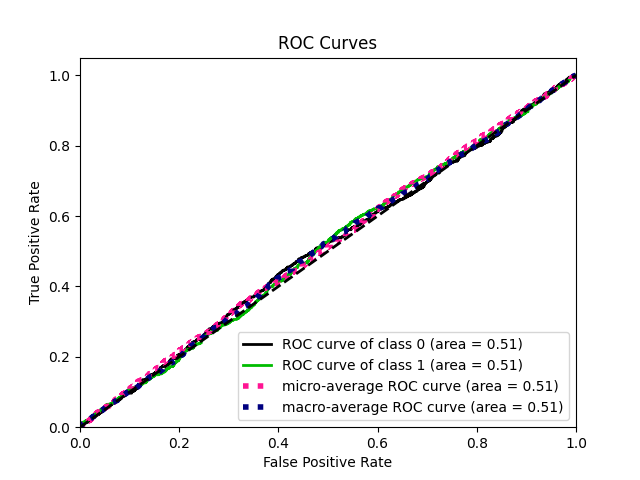
\includegraphics{https://github.com/michaelGuo1204/UThesis/blob/500k_Dataset/docs/media/GNN/True PRS.png?raw=true}
\caption{}
\end{figure}

可以发现,传统PRS模型的风险预测效果较差,AUC仅为0.51,与随机预测相当。这意味着使用PRS模型对骨关节炎的预测几乎没有任何参考意义。这也与Boer{[}5{]}研究中构建的PRS模型结果相符。同时我们也使用了包括决策树算法在内额若干传统机器学习模型对基因型数据进行处理与预测,所得结果与基于PRS的模型无显著差异。本文因此以该PRS模型为基础讨论本文提出模型对预测效果的改善。

\begin{longtable}[]{@{}lll@{}}
\toprule()
指标 & 基于PRS的模型 & 决策树模型 \\
\midrule()
\endhead
auc & 0.51 & 0.50 \\
f1 & 0.45 & 0.29 \\
accuracy & 0.52 & 0.51 \\
precision & 0.50 & 0.50 \\
recall & 0.41 & 0.21 \\
\bottomrule()
\end{longtable}

\hypertarget{ux7279ux5f81ux7b5bux9009ux65b9ux6cd5ux5bf9ux6bd4}{%
\subsubsection{特征筛选方法对比}\label{ux7279ux5f81ux7b5bux9009ux65b9ux6cd5ux5bf9ux6bd4}}

之前的讨论中我们提到,特征筛选对于特征数与样本数之比较高的数据集有着很好的提高模型性能的效果。本文也因此提到了两种特征筛选方法------基于卡方的样本筛选与基于支持向量机的样本筛选。对于使用同样超参数的决策树模型,我们输入使用不同特征筛选方式处理后的数据集并比较两种特征筛选方法对模型效果的影响。结果如下表。

\begin{longtable}[]{@{}lll@{}}
\toprule()
指标 & 经卡方法筛选特征 & 经支持向量机法筛选特征 \\
\midrule()
\endhead
auc & 0.51 & 0.54 \\
f1 & 0.38 & 0.43 \\
accuracy & 0.52 & 0.54 \\
precision & 0.51 & 0.55 \\
recall & 0.29 & 0.35 \\
\bottomrule()
\end{longtable}

可以看出,相较于经卡方法所得特征,经支持向量机法所筛选特征在相同模型上的表现更好,本文因此使用支持向量机法筛选特征。

\hypertarget{ux56feux795eux7ecfux7f51ux7edcux5904ux7406}{%
\subsubsection{图神经网络处理}\label{ux56feux795eux7ecfux7f51ux7edcux5904ux7406}}

将经过支持向量机法筛选所得特征输入本文提出的风险预测模型中进行图估计与图神经网络处理,选择最优的图估计结构后,本文得出以下图神经网络预测结果。

\begin{longtable}[]{@{}lll@{}}
\toprule()
指标 & 图神经网络预测结果 & PRS模型 \\
\midrule()
\endhead
auc & 0.63 & 0.51 \\
f1 & 0.56 & 0.45 \\
accuracy & 0.60 & 0.52 \\
precision & 0.60 & 0.50 \\
recall & 0.53 & 0.41 \\
\bottomrule()
\end{longtable}

可以看出,本文建立的图神经网络较PRS模型及传统机器学习模型性能有了明显改善。证明了图神经网络在处理图数据时的优秀效果

\hypertarget{ux8868ux578bux878dux5408-2}{%
\subsubsection{表型融合}\label{ux8868ux578bux878dux5408-2}}

为进一步增强模型性能,本文引入同骨关节炎密切相关的表型参与风险预测,其给出如下结果。

\begin{longtable}[]{@{}llll@{}}
\toprule()
指标 & 融合表型 & 单纯图神经网络 & PRS模型 \\
\midrule()
\endhead
auc & 0.74 & 0.60 & 0.51 \\
f1 & 0.66 & 0.57 & 0.45 \\
accuracy & 0.67 & 0.58 & 0.52 \\
precision & 0.66 & 0.57 & 0.50 \\
recall & 0.69 & 0.58 & 0.41 \\
\bottomrule()
\end{longtable}

可以看出融合表型之后模型性能有了进一步提升。此时预测AUC以及达到0.74,相较于单纯利用基因型数据的图神经网络预测准确能力显著增强。

\hypertarget{ux56feux4f30ux8ba1ux6548ux679c}{%
\subsection{图估计效果}\label{ux56feux4f30ux8ba1ux6548ux679c}}

\hypertarget{ux4f30ux8ba1ux5668ux5728ux8badux7ec3ux8fc7ux7a0bux4e2dux7684ux6548ux679c}{%
\subsubsection{估计器在训练过程中的效果}\label{ux4f30ux8ba1ux5668ux5728ux8badux7ec3ux8fc7ux7a0bux4e2dux7684ux6548ux679c}}

\hypertarget{ux53efux884cux6027ux9a8cux8bc1}{%
\paragraph{可行性验证}\label{ux53efux884cux6027ux9a8cux8bc1}}

为了验证本文设计图估计器对无结构数据的处理能力,在使用该估计器估计本研究所使用骨关节炎患者基因型数据结构之前,本文先在MNIST数据集上进行测试。MNIST数据集{[}73{]}由若干已标注手写数字图片组成,也是一种无结构数据。我们因此在该数据集上应用我们的模型并将结果加以记录。可以看到,在每个迭代的图估计器工作之后,模型损失有着明显下降,同时分类准确率也有显著提升。这证明了本文提出图估计器对图神经网络在无结构数据上的性能有着明显改善,为后续对骨关节炎患者基因型数据的处理工作提供可行性基础。

\hypertarget{ux5bf9ux7167ux7ec4}{%
\paragraph{对照组}\label{ux5bf9ux7167ux7ec4}}

图估计器的工作过程涉及到图神经网络参数与图结构的循环更新。为了排除多次重启训练对模型性能的潜在影响,我们设计对照组,即使用全连接法构建图矩阵并且每次图神经网络训练之后不更新图结构。并对对照组的模型训练情况做以记录。可以看到,在不更新图结构时,每次迭代中模型损失与准确率的变化趋势基本一致,同时不同迭代末期模型AUC变化不大。因此我们认为模型效果与无图结构更新过程的迭代次数无关。

\hypertarget{ux5b9eux9645ux6570ux636e}{%
\paragraph{实际数据}\label{ux5b9eux9645ux6570ux636e}}

该组试验中我们正式将图估计器与图神经网络运用于骨关节炎患者基因型数据的处理过程中。我们首先使用全连接法构建初始图,在每个迭代中我们训练神经网络并给出数据在该网络下的输出,再将输出作为图估计器的观察值并基于此更新图结构,再将该图结构作为数据的结构重新输入图神经网络中训练。如此迭代若干次,记录模型性能如下。

可以看出,首次迭代中由于使用全连接网络,模型性能变化同对照组中模型相仿。但是在首次迭代结束生成新图结构后并以此进行第二次迭代的图神经网络训练时我们可以发现,训练末期模型损失明显下降,模型准确率明显上升。模型预测能力AUC也有明显提高。最终我们选择预测能力最好的迭代作为最优模型,参与到骨关节炎风险预测过程之中。

\hypertarget{ux56feux4f30ux8ba1ux5668ux5de5ux4f5cux8fc7ux7a0bux5206ux6790}{%
\subsubsection{图估计器工作过程分析}\label{ux56feux4f30ux8ba1ux5668ux5de5ux4f5cux8fc7ux7a0bux5206ux6790}}

\hypertarget{ux805aux7c7bux53c2ux6570ux9009ux62e9}{%
\paragraph{聚类参数选择}\label{ux805aux7c7bux53c2ux6570ux9009ux62e9}}

在讨论图估计器时我们提到,图估计器在输入观察值的同时还需要人工选择聚类参数\(k\)以初始化变分参数,且该聚类参数会对估计结果产生直接影响,该影响可通过整合分类似然评估。为了选择最优聚类参数,我们计算了使用一定范围内的聚类参数时的模型整合分类似然,结果如下。

可以发现,\(k\)取6时模型的整合分类似然最低,性能最好。同时我们考虑了在使用该范围内参数时变分期望最大化算法所给出的证据下界ELBO,我们发现虽然\(k\)取6的组证据下界并非最高,但是同其他组相比也处于高位。因此我们将\(k\)定为6并估计该参数下可能的图结构。

\hypertarget{ux751fux6210ux56feux7ed3ux6784ux5206ux6790}{%
\paragraph{生成图结构分析}\label{ux751fux6210ux56feux7ed3ux6784ux5206ux6790}}

根据前文对变分期望最大化算法的讨论我们可以发现,\(k\)取6意味着最终生成的图结构可以分为6簇。为了探究该网络结构以及其潜藏的信息,我们将估计图结构中的节点依照其所属的簇加以归类并表示如下图。

我们同时将计算所得的簇与簇之间的关系表示如下。可以发现,簇3与簇4、簇2与簇6之间存在着很强的相关信号。且簇6与除簇1,2之外的其它簇关联都不强。我们同时发现簇3、5之间也存在一相关信号。初此以外数学分析无法从该图中获取更多信息,我们因此需要结合图中节点的生物学意义对该图结构与簇关系加以分析。

\hypertarget{ux7ed3ux5408ux8868ux578bux5206ux6790}{%
\paragraph{结合表型分析}\label{ux7ed3ux5408ux8868ux578bux5206ux6790}}

为了进一步探究生成图结构的生物学意义,我们需要了解其中节点,也就是SNP位点对人的不同表型的贡献。同GWAS研究类似的,全表型关联研究(Phenome-wide
Association
Study,PheWAS)主要研究某一SNP位点与已知性状的关联{[}74{]},因此我们对图中每个节点进行PheWAS研究。我们对节点的研究主要在GWASATLAS数据库内进行{[}75{]},该数据库包含了在UKB数据上进行的对3302个表型的约4756个GWAS研究,可以较为全面地展现SNP位点对表型的影响。对于每个SNP,我们编写爬虫由数据库获取与其相关的表型以及该相关的统计学显著性,经过统计学显著性筛选(\(p<10^{-5}\))后将与每个SNP相关的表型按照领域分为25类。对于每个簇,我们统计簇内SNP位点对每类性状的关联并进行簇内标准化,得出如下热图。

\begin{figure}
\centering
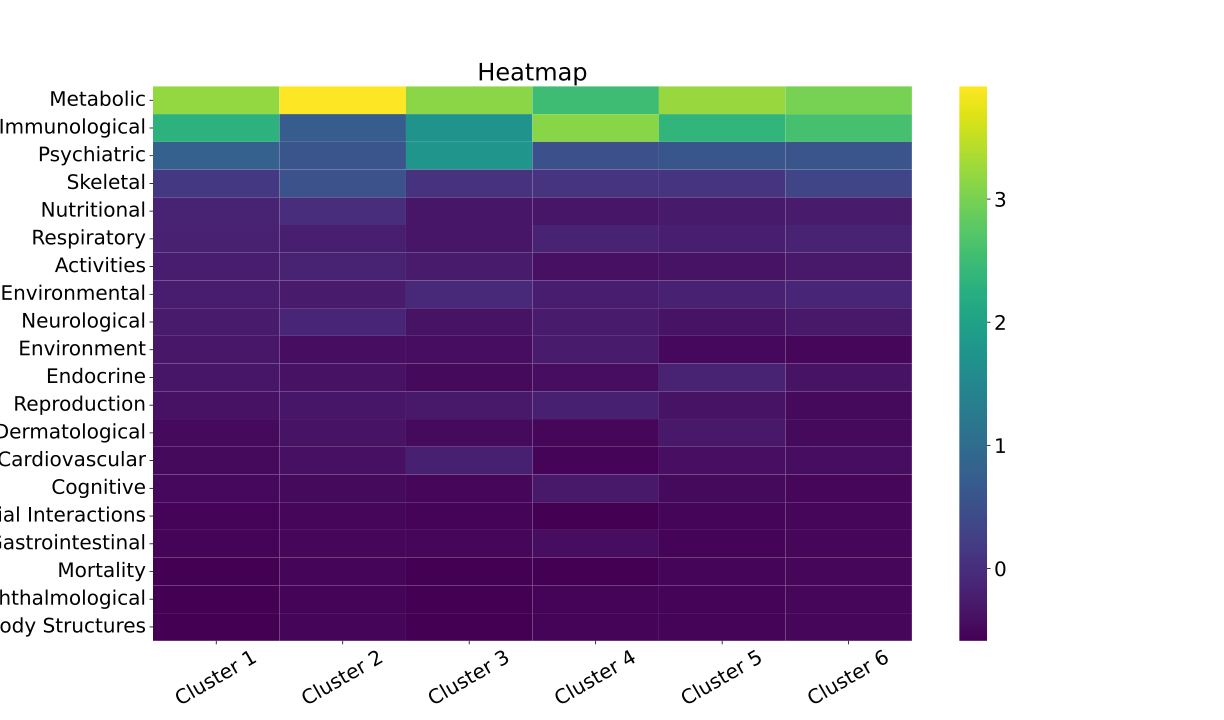
\includegraphics{G:/bili/Lernen/UThesis/EM/VEM/Cluster/heatmap_col.svg}
\caption{}
\end{figure}

可以看出,每个簇内与簇内SNP相关联程度最高的表型均集中在代谢与免疫领域,这也与骨关节炎本身炎症性质相关。为了能近一步分析簇间差异,我们还对每个领域内关联进行簇间标准化,得到如下热图。

\begin{figure}
\centering
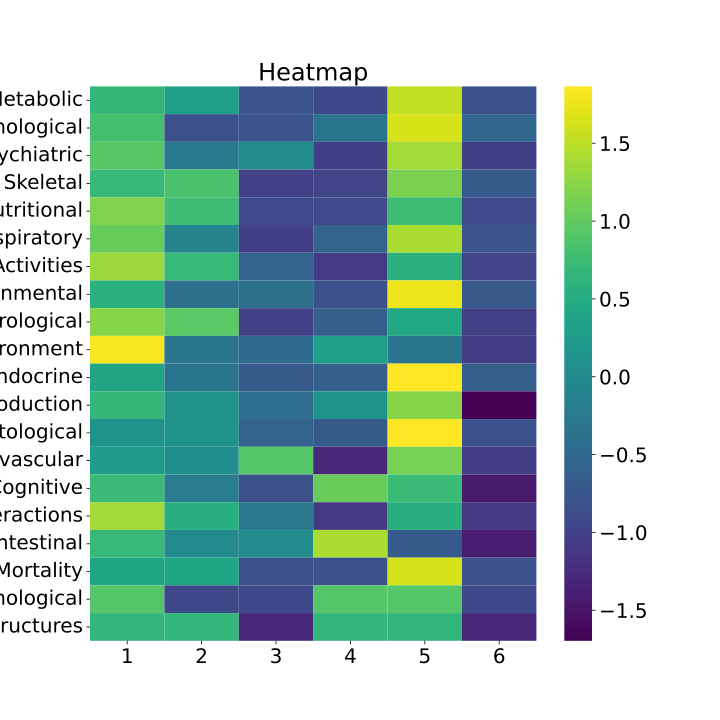
\includegraphics{G:/bili/Lernen/UThesis/EM/VEM/Cluster/heatmap_row.svg}
\caption{}
\end{figure}

相较于簇内标准化,我们可以从此图中发现簇间的明显差异,尤其是簇1、5在环境、内分泌、免疫等领域同其他簇存在明显差异。本文因此对该两簇进行深入分析

同其他簇相同,与簇一内SNP位点相关表型主要集中在代谢与免疫领域。但是我们从热图中发现簇一有着较强的环境相关信号。我们对该环境相关信号加以统计,结果如表所示。出乎我们意料的是,与簇一内SNP相关的环境相关表型出现了受教育程度、工作是否涉及重体力劳动等看起来与骨关节炎毫不相干的性状。但是,在查阅文献{[}77{]}后我们了解到,骨关节炎作为一种退化性疾病有可能与关节过度磨损相关。因此我们做出猜测,受教育程度较低的个体趋向于从事体力型劳动,导致关节加速磨损,最终导致骨关节炎的发生。而该簇内的SNP可能在受到这种环境影响时更易导致骨关节炎的发生。我们猜测该簇内SNP可能与环境因素导致关节磨损继而导致的骨关节炎相关。

\begin{longtable}[]{@{}lll@{}}
\toprule()
领域 & 表型 & 计数 \\
\midrule()
\endhead
Environment & Educational attainment & 10 \\
Environment & Education - Qualifications & 3 \\
Environment & Attendance/disability/mobility allowance: Blue badge &
1 \\
Environment & Job involves heavy manual or physical work & 1 \\
Environment & Maternal smoking around birth & 1 \\
\bottomrule()
\end{longtable}

我们也对簇五进行了类似分析,相较于其他簇,簇五在免疫、内分泌、皮肤病领域有着很强相关。我们对这些领域内的典型性状加以统计得到表。可以看出,簇五内的SNP与二型糖尿病、巨噬细胞、白细胞与粒细胞计数相关表型都存在着相关。二型糖尿病是一种由于机体胰岛素抗性而生成的糖尿病,其主要由超重乃至肥胖而导致。{[}78{]}而肥胖导致的高血脂又会诱发体内免疫系统包括巨噬细胞与粒细胞的激活。{[}79{]}这也与簇内的观察一致,因此我们猜测簇五内的SNP位点主要与个体自身肥胖导致的糖尿病与超重继而诱发的自身型骨关节炎相关。

\begin{longtable}[]{@{}lll@{}}
\toprule()
域 & 表型 & 计数 \\
\midrule()
\endhead
Endocrine & Type 2 Diabetes & 25 \\
Immunological & Myeloid white cell count (three-way meta) & 14 \\
Immunological & White blood cell count (three-way meta) & 14 \\
Immunological & Granulocyte count (three-way meta) & 13 \\
Dermatological & Male pattern baldness & 10 \\
\bottomrule()
\end{longtable}

以上我们通过对图估计生成图结构的分析将输入的致病SNP分为六簇并对其中两个典型簇进行具体生物学意义分析。同时根据两簇内SNP的相关性状提出了骨关节炎的两种诱因,即由环境因素导致关节过度磨损诱发的骨关节炎以及由于超重诱发的自身型骨关节炎。而这类分析是传统机器学习模型所无法实现的,这也进一步印证了图神经网络在学习数据深度信息时的出众能力。

\hypertarget{ux56feux89e3ux91caux5668ux7ed3ux679cux6848ux4f8bux5206ux6790}{%
\subsection{图解释器结果案例分析}\label{ux56feux89e3ux91caux5668ux7ed3ux679cux6848ux4f8bux5206ux6790}}

我们之前提到本风险预测模型中的图解释器能对产生预测结果的原因,即输入基因型图中同预测结果相关的最大子图,加以分析与计算。本节通过模型对UKB数据库中一个案的分析结果展示该能力。本文从UKB数据库中选取样本(UID=5125713),并将其基因型数据根据图估计器给出的最佳图结构转为图数据。利用训练好的图神经网络模型对该图进行处理,预测结果为该样本有很高概率患骨关节炎。我们将该预测结果与模型输入图解释器中,最终图解释器给出如下相关子图。

\begin{figure}
\centering
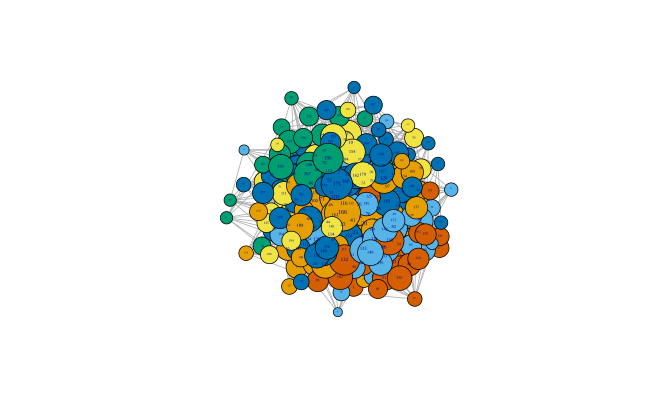
\includegraphics{G:/bili/Lernen/UThesis/EM/VEM/Explain_5125713/0.3.svg}
\caption{}
\end{figure}

在该子图中,边的权重为该关联对预测值的贡献,权重越高代表该边对预测值的生成越``重要''。我们将该图按照边的权重进行稀疏化,得到如下系列子图。可以看到,随着权重阈值的不断提升,子图的骨干逐渐显现,而该主干则主要由簇一、五中的节点构成。上一节的分析中我们提到簇五中所含位点可能与二型糖尿病相关,我们因此推测该个体可能由肥胖造成的关节过度磨损诱发骨关节炎,同时该患者可能合并二型糖尿病。我们从UKB数据库中提取患者其他表型。

\begin{longtable}[]{@{}lll@{}}
\toprule()
UKB-ID & 表型 & 值 \\
\midrule()
\endhead
31 & 性别 & 男 \\
48 & 腰围 & 113 \\
49 & 胯围 & 121 \\
2443 & 确诊糖尿病 & 是 \\
21001 & BMI & 35.2 \\
23098 & 体重 & 105.5 \\
23099 & 体脂率 & 46.1 \\
\bottomrule()
\end{longtable}

患者实际BMI为35.2,体脂率为46\%,已为肥胖体型,并且合并确诊糖尿病。可以看出,患者实际情况同我们根据图结构以及图解释器做出的解释一致。体现了本文提出模型除高效预测骨关节炎风险之外对疾病分型以辅助治疗的能力。

\hypertarget{ux672cux7ae0ux5c0fux7ed3-3}{%
\subsection{本章小结}\label{ux672cux7ae0ux5c0fux7ed3-3}}

本章对本文搭建的骨关节炎风险预测模型的预测准确性通过若干指标加以评估并同现有的常见疾病风险预测模型算法进行比较,发现本文搭建模型较传统PRS方法与机器学习算法而言在准确性上有着显著提高,已可作为临床辅助工具参与骨关节炎的早期诊断。本章同时对图估计器的工作过程加以记录与展示,一方面验证了算法的可行性;另一方面也证实了图估计器可以显著改善无结构数据在图神经网络中的表现。为了进一步挖掘潜藏在估计器所得图结构中的信息,本章还结合图估计器输出数学模型与图中节点的PheWAS研究结果对图中的簇聚节点之间关系加以分析并且识别出了两个典型簇,并且根据典型簇内节点信息提出了关节炎的两种诱因。最后本章利用模型解释器进行案例分析,在给出预测结果的同时还利用解释器的结果与识别出的典型簇预测了疾病的分型。以上内容完整展现了本模型作为高效准确可解释骨关节炎风险预测模型的功能与性能。

\hypertarget{ux603bux7ed3ux4e0eux5c55ux671b}{%
\section{总结与展望}\label{ux603bux7ed3ux4e0eux5c55ux671b}}

\hypertarget{ux5de5ux4f5cux603bux7ed3}{%
\subsection{工作总结}\label{ux5de5ux4f5cux603bux7ed3}}

构建高效可解释骨关节炎对骨关节炎的早期诊断与防治有着重要的意义。本文首先根据目前已发表的GWAS研究及公共数据库UK
BioBank获取患者表型与基因型数据并进行数据预处理;之后构建了包括图结构估计器、图卷积神经网络、表型信息融合与图解释器四个模块在内的骨关节炎风险预测模型;最后本文对该模型的性能以及预测结果进行了进一步的分析和解读,继而对模型的预测准确性,可解释性等指标进行评估。本文对主要完成的工作总结如下。

\begin{enumerate}
\def\labelenumi{\arabic{enumi}.}
\item
  获取骨关节患者表型与基因型:本文从UKB数据库获取了13709名个体的基因型与表型数据。本文同时根据现有GWAS研究对于每个个体选取8687个基因型位点作为感兴趣位点并进行预处理。为了改善模型性能,降低计算复杂度,本文还对该数据进行了特征筛选。
\item
  构建骨关节炎风险预测模型:本文根据模型所处理数据以及需求设计了包括图结构估计器、图神经网络、表型信息融合与图解释器四个模块在内的骨关节炎风险预测模型。图结构估计器主要基于变分期望最大化算法将输入的无结构数据转化为可被图神经网络处理的图数据。图神经网络以谱图神经网络中的切比雪夫层为核心对估计器产生的图数据加以处理并给出风险预测。表型信息融合模块通过引入表型信息作为协变量进一步提高模型性能。图解释器则基于网络输入数据与预测结果对输入数据中对预测结果贡献最大的子图加以计算。以上模块共同构成了本文提出的骨关节炎风险预测模型。
\item
  验证骨关节风险预测模型功能与性能:本文对提出模型的风险预测性能进行了评估、对图估计器产生的图结构加以解释,还利用图解释器进行案例分析。风险预测性能评估方面本文选择了一系列指标对模型的预测性能加以评估,并同包括PRS模型、常见机器学习算法在内的传统疾病风险预测模型相比较。证明本模型较传统疾病风险预测模型而言有着十分明显的性能改善。同时本文对图估计器的工作过程加以分析与展示,同时结合图中节点生物学意义对图估计器产生图结构加以分析。分析中本文识别出了图结构中的两类典型簇并根据节点PheWAS研究对该簇对于骨关节炎的意义加以研究。本文还选择UKB数据库中一个体进行案例分析,演示模型工作效果,展现了模型一方面给出可靠预测结果;另一方面对可能病因揭示的能力。
\end{enumerate}

\hypertarget{ux5c55ux671b}{%
\subsection{展望}\label{ux5c55ux671b}}

虽然本文所提出风险预测模型在给出可信预测结果的同时兼具可解释性,但是本文中还存在若干问题需要进一步研究

\begin{enumerate}
\def\labelenumi{\arabic{enumi}.}
\item
  模型超参数与结构还存在调整空间:本模型中四个模块都有着数量较多的决定模型性能的超参数,由于时间限制本文未能对这些超参数进行细致调整,可能对最终模型的性能产生不利影响。后续研究中仍要对其中一些参数加以分析调整以求继续提高模型性能。同时随着图神经网络研究的快速发展,本研究进行之时不断有效果更好的图卷积方式出现,后续研究中还需基于这些研究对图卷积层进行优化。
\item
  图估计器仍需继续研究:为了简化问题,本模型图估计器所生成的图结构中各边的权重一致。但是现实生活中的图数据中各边权重通常不一致,并且有着具体意义,忽略该权重意味着潜藏信息的损失。如何通过参数描述各边的权重并通过算法估计该参数仍需后续研究。
\item
  图估计产生图结构仍需进一步分析:本研究中图估计器生成的图结构共分为六簇,但是由于SNP位点生物学意义的复杂性,本文只对其中两簇进行了浅显的分析,并且没有对簇内节点之间与簇与簇之间的关联加以深入解释。后续研究中仍要对产生该结构的具体原因与意义加以具体分析
\end{enumerate}

{[}1{]}:Martel-Pelletier, Johanne; Barr, Andrew J.; Cicuttini, Flavia
M.; Conaghan, Philip G.; Cooper, Cyrus; Goldring, Mary B.; Goldring,
Steven R.; Jones, Graeme; Teichtahl, Andrew J.; Pelletier, Jean-Pierre
(2016). \emph{Osteoarthritis. Nature Reviews Disease Primers, 2(),
16072--.} doi:10.1038/nrdp.2016.72

{[}2{]}: Collaborators, G. B. D. D., Injury, I., \& Prevalence. (2018).
Global, regional, and national incidence, prevalence, and years lived
with disability for 354 diseases and injuries for 195 countries and
territories, 1990-2017: a systematic analysis for the Global Burden of
Disease Study 2017.
\url{https://doi.org/10.1016/S0140-6736(18)32279-7}'{]}

{[}3{]}:Vos, T. et al. Years lived with disability (ylds) for 1160
sequelae of 289 diseases and injuries 1990-2010: a systematic analysis
for the global burden of disease study 2010. Lancet 380, 2163--2196
(2012).

{[}4{]}: Hiligsmann, M. et al. Health economics in the feld of
osteoarthritis: an expert's consensus paper from the european society
for clinical and economic aspects of osteoporosis and osteoarthritis
(ESCEO). Semin. Arthritis Rheum. 43, 303--313 (2013).

{[}5{]}:Boer, C. G., Hatzikotoulas, K., Southam, L., Stefánsdóttir, L.,
Zhang, Y., Coutinho de Almeida, R., Wu, T. T., Zheng, J., Hartley, A.,
Teder-Laving, M., Skogholt, A. H., Terao, C., Zengini, E., Alexiadis,
G., Barysenka, A., Bjornsdottir, G., Gabrielsen, M. E., Gilly, A.,
Ingvarsson, T., . . . Zeggini, E. (2021). Deciphering osteoarthritis
genetics across 826,690 individuals from 9 populations. \emph{Cell},
\emph{184}(18), 4784-4818.e4717.
\url{https://doi.org/10.1016/j.cell.2021.07.038}

{[}6{]}:Cooper, C. et al. Risk factors for the incidence and progression
of radiographic knee osteoarthritis. Arthritis Rheum. 43, 995--1000
(2000).

{[}7{]}:Zhang, Y. et al. Methodologic challenges in studying risk
factors for progression of knee osteoarthritis. Arthritis Care Res.
(Hoboken) 62, 1527--1532 (2010)

{[}8{]}:Veronese, N. et al. Osteoarthritis and mortality: a prospective
cohort study and systematic review with meta-analysis. Semin. Arthritis
Rheum. http:// dx.doi.org/10.1016/j.semarthrit.2016.04.002 (2016)

{[}9{]}:Styrkarsdottir, U., Lund, S.H., Thorleifsson, G. \emph{et al.}
Meta-analysis of Icelandic and UK data sets identifies missense variants
in \emph{SMO}, \emph{IL11}, \emph{COL11A1} and 13 more new loci
associated with osteoarthritis. \emph{Nat Genet} \textbf{50,} 1681--1687
(2018). \url{https://doi.org/10.1038/s41588-018-0247-0}

{[}10{]}:Tachmazidou, I., Hatzikotoulas, K., Southam, L. \emph{et al.}
Identification of new therapeutic targets for osteoarthritis through
genome-wide analyses of UK Biobank data. \emph{Nat Genet} \textbf{51,}
230--236 (2019). \url{https://doi.org/10.1038/s41588-018-0327-1}

{[}11{]}:Zengini, E., Hatzikotoulas, K., Tachmazidou, I. \emph{et al.}
Genome-wide analyses using UK Biobank data provide insights into the
genetic architecture of osteoarthritis. \emph{Nat Genet} \textbf{50,}
549--558 (2018). \url{https://doi.org/10.1038/s41588-018-0079-y}

{[}12{]}:Choi, Shing Wan; Mak, Timothy Shin-Heng; O’Reilly, Paul F.
(2020). \emph{Tutorial: a guide to performing polygenic risk score
analyses. Nature Protocols, (), --.} doi:10.1038/s41596-020-0353-1

{[}13{]}: Jostins, L., and Barrett, J. C. (2011). Genetic risk
prediction in complex disease. \emph{Hum. Mol. Genet.} 20, 182--188.
doi: 10.1093/hmg/ddr378

{[}14{]}: Wray, N. R., Lee, S. H., Mehta, D., Vinkhuyzen, A. A. E.,
Dudbridge, F., and Middeldorp, C. M. (2014). Research review: polygenic
methods and their application to psychiatric traits. \emph{J. Child
Psychol. Psychiatry Allied Discip.} 55, 1068--1087. doi:
10.1111/jcpp.12295

{[}15{]}:So, H. C., Sham, P. C., and Valencia, A. (2017). Exploring the
predictive power of polygenic scores derived from genome-wide
association studies: a study of 10 complex traits. \emph{Bioinformatics}
33, 886--892. doi: 10.1093/bioinformatics/btw745

{[}16{]}: Capriotti, E., Calabrese, R., and Casadio, R. (2006).
Predicting the insurgence of human genetic diseases associated to single
point protein mutations with support vector machines and evolutionary
information. \emph{Bioinformatics} 22, 2729--2734. doi:
10.1093/bioinformatics/btl423

{[}17{]}:Cruz, J. A., and Wishart, D. S. (2006). Applications of machine
learning in cancer prediction and prognosis. \emph{Cancer Inform.} 2,
59--77. doi: 10.1177/117693510600200030

{[}18{]}:Palaniappan, S., and Awang, R. (2008). ``Intelligent heart
disease prediction system using data mining techniques,'' in
\emph{Proceedings of the 2008 IEEE/ACS Int. Conf. Comput. Syst. Appl},
(Doha), 108--115. doi: 10.1109/AICCSA.2008.4493524

{[}19{]}:Yu, W. (2010). Application of support vector machine modeling
for prediction of common diseases: the case of diabetes and
pre-diabetes. \emph{BMC Med. Inform. Decis. Mak.} 10:16. doi:
10.1186/1472-6947-10-16

{[}20{]}:Zhang, D., and Shen, D. (2012). Multi-modal multi-task learning
for joint prediction of multiple regression and classification variables
in Alzheimer's disease. \emph{Neuroimage} 59, 895--907. doi:
10.1016/j.neuroimage.2011.09.069

{[}21{]}:López, B., Torrent-Fontbona, F., Viñas, R., and Fernández-Real,
J. M. (2017). Single nucleotide polymorphism relevance learning with
random forests for type 2 diabetes risk prediction. \emph{Artif. Intell.
Med.} 85, 43--49. doi: 10.1016/j.artmed.2017.09.005

{[}22{]}:Montañez, C. A. C., Fergus, P., and Chalmers, C. (2015). ``Deep
learning classification of polygenic obesity using genome wide
association study SNPs,'' in \emph{Proceedings of the 2018 International
Joint Conference on Neural Networks (IJCNN)}, (Budapest).

{[}23{]}:M. M. Bronstein, J. Bruna, Y. LeCun, A. Szlam and P. Van der
Gheynst, "Geometric deep learning: Going beyond Euclidean data",
\emph{IEEE Signal Process. Mag.}, vol. 34, no. 4, pp. 18-42, Jul. 2017.

{[}24{]}:A. Sperduti and A. Starita, "Supervised neural networks for the
classification of structures", \emph{IEEE Trans. Neural Netw.}, vol. 8,
no. 3, pp. 714-735, May 1997.

{[}25{]}:M. Gori, G. Monfardini and F. Scarselli, "A new model for
learning in graph domains", \emph{Proc. IEEE Int. Joint Conf. Neural
Netw.}, vol. 2, pp. 729-734, Aug. 2005.

{[}26{]}:K. Xu, W. Hu, J. Leskovec and S. Jegelka, "How powerful are
graph neural networks", \emph{Proc. ICLR}, pp. 1-17, 2019.

{[}27{]}:P. Velickovic, G. Cucurull, A. Casanova, A. Romero, P. Lio and
Y. Bengio, "Graph attention networks", \emph{Proc. ICLR}, pp. 1-12,
2017.

{[}28{]}:J. Atwood and D. Towsley, "Diffusion-convolutional neural
networks", \emph{Proc. NIPS}, pp. 1993-2001, 2016.

{[}29{]}:T. N. Kipf and M. Welling, "Semi-supervised classification with
graph convolutional networks", \emph{Proc. ICLR}, pp. 1-14, 2017.

{[}30{]}:M. Defferrard, X. Bresson and P. Van der Gheynst,
"Convolutional neural networks on graphs with fast localized spectral
filtering", \emph{Proc. NIPS}, pp. 3844-3852, 2016.

{[}31{]}:R. Li, S. Wang, F. Zhu and J. Huang, "Adaptive graph
convolutional neural networks", \emph{Proc. AAAI}, pp. 3546-3553, 2018.

{[}32{]}:Veselkov, K., Gonzalez, G., Aljifri, S., Galea, D., Mirnezami,
R., Youssef, J., Bronstein, M., \& Laponogov, I. (2019). HyperFoods:
Machine intelligent mapping of cancer-beating molecules in foods.
\emph{Scientific Reports}, \emph{9}(1), 9237.
\url{https://doi.org/10.1038/s41598-019-45349-y}

{[}33{]}:Knyazev, B., Lin, X., Amer, M. R., \& Taylor, G. W. (2018).
Spectral Multigraph Networks for Discovering and Fusing Relationships in
Molecules. \emph{arXiv:1811.09595 {[}cs, stat{]}}.
\url{http://arxiv.org/abs/1811.09595}

{[}34{]}:Yan, S., Xiong, Y., \& Lin, D. (2018). Spatial Temporal Graph
Convolutional Networks for Skeleton-Based Action Recognition.
\emph{arXiv:1801.07455 {[}cs{]}}. \url{http://arxiv.org/abs/1801.07455}

{[}35{]}:Ghosal, S., Pergola, G., Chen, Q., Goldman, A. L., Ulrich, W.,
Weinberger, D. R., \& Venkataraman, A. (2021). \emph{A Biologically
Interpretable Graph Convolutional Network to Link Genetic Risk Pathways
and Neuroimaging Phenotypes of Disease}.
\url{https://www.biorxiv.org/content/10.1101/2021.05.28.446066v1}

{[}36{]}:Ying, R., Bourgeois, D., You, J., Zitnik, M., \& Leskovec, J.
(2019). GNNExplainer: Generating Explanations for Graph Neural Networks.
\emph{arXiv:1903.03894 {[}cs, stat{]}}.
\url{http://arxiv.org/abs/1903.03894}

{[}37{]}:Sudlow, C. et al. UK Biobank: an open access resource for
identifying the causes of a wide range of complex diseases of middle and
old age. \emph{PLoS Med.} \textbf{12}, e1001779 (2015).

{[}39{]}:Zhongsheng Chen, Michael Boehnke, Xiaoquan Wen, Bhramar
Mukherjee, Revisiting the genome-wide significance threshold for common
variant GWAS, \emph{G3 Genes\textbar Genomes\textbar Genetics}, Volume
11, Issue 2, February 2021, jkaa056,
\url{https://doi.org/10.1093/g3journal/jkaa056}

{[}40{]}: Wilk, M.B.; Gnanadesikan, R. (1968), "Probability plotting
methods for the analysis of data", \emph{Biometrika}, Biometrika Trust,
\textbf{55} (1): 1--17,
\href{https://en.wikipedia.org/wiki/Doi_(identifier)}{doi}:\href{https://doi.org/10.1093\%2Fbiomet\%2F55.1.1}{10.1093/biomet/55.1.1},
\href{https://en.wikipedia.org/wiki/JSTOR_(identifier)}{JSTOR}
\href{https://www.jstor.org/stable/2334448}{2334448},
\href{https://en.wikipedia.org/wiki/PMID_(identifier)}{PMID}
\href{https://pubmed.ncbi.nlm.nih.gov/5661047}{5661047}.

{[}41{]}:Marees, A. T., de Kluiver, H., Stringer, S., Vorspan, F.,
Curis, E., Marie-Claire, C., \& Derks, E. M. (2018). A tutorial on
conducting genome-wide association studies: Quality control and
statistical analysis. \emph{International journal of methods in
psychiatric research}, \emph{27}(2), e1608.
\url{https://doi.org/10.1002/mpr.1608}

{[}42{]}:Holly Janes, Margaret Pepe, The optimal ratio of cases to
controls for estimating the classification accuracy of a biomarker,
\emph{Biostatistics}, Volume 7, Issue 3, July 2006, Pages 456--468,
\url{https://doi.org/10.1093/biostatistics/kxj018}

{[}43{]}:Tibshirani, R. (1996). Regression shrinkage and selection via
the Lasso. Journal of the Royal Statistical Society, Series B, 58:1,
267--288

{[}44{]}:Bradley, P. S., \& Mangasarian, O. L. (1998). Feature selection
via concave minimization and support vector machines. In J. Shavlik
(Ed.), Proceedings of the 15th international conference on machine
learning (pp. 82-- 90). San Francisco, CA: Morgan Kaufmann.

{[}45{]}:Jiafeng Hu, Reynold Cheng, Zhipeng Huang, Yixang Fang, and
Siqiang Luo. 2017. On Embedding Uncertain Graphs. In \emph{Proceedings
of the 2017 ACM on Conference on Information and Knowledge Management}
(\emph{CIKM '17}). Association for Computing Machinery, New York, NY,
USA, 157--166. \url{https://doi.org/10.1145/3132847.3132885}

{[}48{]}: {[}Preparata and Shamos, 1985{]} F. P. Preparata and M. I.
Shamos. Computational Geometry: An Introduction. Springer, 1985.

{[}49{]}:{[}Bentley et al., 1977{]} J. L. Bentley, D. F. Stanat, and E.
H. Williams Jr. The Complexity of Finding Fixed-Radius Near Neighbors.
Inf. Process. Lett., 1977.

{[}50{]}: Holland, Paul W; Laskey, Kathryn Blackmond; Leinhardt, Samuel
(1983). \href{https://doi.org/10.1016/0378-8733(83)90021-7}{"Stochastic
blockmodels: First steps"}.
\emph{\href{https://en.wikipedia.org/wiki/Social_Networks}{Social
Networks}}. \textbf{5} (2): 109--137.
\href{https://en.wikipedia.org/wiki/Doi_(identifier)}{doi}:\href{https://doi.org/10.1016\%2F0378-8733(83)90021-7}{10.1016/0378-8733(83)90021-7}.
\href{https://en.wikipedia.org/wiki/ISSN_(identifier)}{ISSN}
\href{https://www.worldcat.org/issn/0378-8733}{0378-8733}. Retrieved
2021-06-16.

{[}51{]}:Y. Zhang, S. Pal, M. Coates, and D. Üstebay. Bayesian Graph
Convolutional Neural Networks for Semi-Supervised Classification. In
AAAI, 2019.

{[}52{]}:{[}Elinas et al., 2020{]} P. Elinas, E. V. Bonilla, and L. C.
Tiao. Variational Inference for Graph Convolutional Networks in the
Absence of Graph Data and Adversarial Settings. In NeurIPS, 2020.

{[}54{]}:Ruijia Wang, Shuai Mou, Xiao Wang, Wanpeng Xiao, Qi Ju, Chuan
Shi, and Xing Xie. 2021. Graph Structure Estimation Neural Networks. In
Proceedings of the Web Conference 2021(WWW '21). Association for
Computing Machinery, New York, NY, USA, 342--353.
\url{https://doi.org/10.1145/3442381.3449952}

{[}55{]}:Dempster, A. P., Laird, N. M., and Rubin, D. B. (1977). Maximum
likelihood from incomplete data via the EM algorithm. Journal of the
Royal Statistical Society. Series B, 39, 1--38.

{[}56{]}:Jordan, M. I., Ghahramani, Z., Jaakkola, T. S., and Saul, L. K.
(1999). An introduction to variational methods for graphical models.
Machine learning, 37, 183--233.

{[}57{]}:Jaakkola, T. S., and Jordan, M. I. (2000). Bayesian parameter
estimation via variational methods. Statistics and Computing, 10,
25--37.

{[}58{]}:
\href{https://en.wikipedia.org/wiki/Johan_Jensen_(mathematician)}{Jensen,
J. L. W. V.} (1906). \href{https://zenodo.org/record/2371297}{"Sur les
fonctions convexes et les inégalités entre les valeurs moyennes"}.
\emph{\href{https://en.wikipedia.org/wiki/Acta_Mathematica}{Acta
Mathematica}}. \textbf{30} (1): 175--193.
\href{https://en.wikipedia.org/wiki/Doi_(identifier)}{doi}:\href{https://doi.org/10.1007\%2FBF02418571}{10.1007/BF02418571}

{[}59{]}:D. G. Tzikas, A. C. Likas, and N. P. Galatsanos, The
Variational Approximation for Bayesian Inference, IEEE Signal Processing
Magazine, Nov 2008

{[}60{]}:R.M. Neal and G.E. Hinton, A view of the EM algorithm that
justifies incremental, sparse and other variants, Learning in Graphical
Models, 1998

{[}61{]}:Abir El Haj. Stochastics blockmodels, classifications and
applications. Modeling and Simulation. Université de Poitiers;
Université Libanaise, 2019. English. ffNNT : 2019POIT2300ff.
fftel-02926379f

{[}62{]}:Abir El Haj, Yousri Slaoui, Pierre-Yves Louis, Zaher Khraibani.
Estimation in a Binomial Stochastic Blockmodel for a Weighted Graph by a
Variational Expectation Maximization Algorithm. Communications in
Statistics - Simulation and Computation, Taylor \& Francis, 2020,
ff10.1080/03610918.2020.1743858ff. ffhal-02271491v1f

{[}63{]}: Schwarz, Gideon E. (1978), "Estimating the dimension of a
model",
\emph{\href{https://en.wikipedia.org/wiki/Annals_of_Statistics}{Annals
of Statistics}}, \textbf{6} (2): 461--464,
\href{https://en.wikipedia.org/wiki/Doi_(identifier)}{doi}:\href{https://doi.org/10.1214\%2Faos\%2F1176344136}{10.1214/aos/1176344136},
\href{https://en.wikipedia.org/wiki/MR_(identifier)}{MR}
\href{https://www.ams.org/mathscinet-getitem?mr=0468014}{0468014}.

{[}64{]}:Daudin, J. J., Picard, F., and Robin, S. (2008). A mixture
model for random graphs. Statistics and computing, 2, 173--183.

{[}66{]}: Proakis, John G.; Manolakis, Dimitri G. (1996),
\href{https://archive.org/details/digitalsignalpro00proa}{\emph{Digital
Signal Processing: Principles, Algorithms and Applications}} (3 ed.),
New Jersey: Prentice-Hall International, p. 297,
\href{https://en.wikipedia.org/wiki/Bibcode_(identifier)}{Bibcode}:\href{https://ui.adsabs.harvard.edu/abs/1996dspp.book.....P}{1996dspp.book.....P},
\href{https://en.wikipedia.org/wiki/ISBN_(identifier)}{ISBN}
\href{https://en.wikipedia.org/wiki/Special:BookSources/9780133942897}{9780133942897},
sAcfAQAAIAAJ

{[}67{]}:Stahlschmidt, S. R., Ulfenborg, B., \& Synnergren, J. (2022).
Multimodal deep learning for biomedical data fusion: a review.
\emph{Briefings in Bioinformatics}, \emph{23}(2), bbab569.
\url{https://doi.org/10.1093/bib/bbab569}

{[}69{]}: Gaudillo J, Rodriguez JJR, Nazareno A, Baltazar LR, Vilela J,
Bulalacao R, et al. (2019) Machine learning approach to single
nucleotide polymorphism-based asthma prediction. PLoS ONE 14(12):
e0225574. \url{https://doi.org/10.1371/journal.pone.0225574}

{[}70{]}: Fawcett, Tom (2006); \emph{An introduction to ROC analysis},
Pattern Recognition Letters, 27, 861--874.

{[}71{]}:Zou, K.H., O'Malley, A.J., Mauri, L. (2007). Receiver-operating
characteristic analysis for evaluating diagnostic tests and predictive
models. \emph{Circulation}, 6;115(5):654--7.

{[}72{]}:Naaman, Michael (2021).
\href{https://www.sciencedirect.com/science/article/pii/S016771522100050X}{"On
the tight constant in the multivariate Dvoretzky-Kiefer-Wolfowitz
inequality"}. \emph{Statistics and Probability Letters}. \textbf{173}:
109088.
\href{https://en.wikipedia.org/wiki/Doi_(identifier)}{doi}:\href{https://doi.org/10.1016\%2Fj.spl.2021.109088}{10.1016/j.spl.2021.109088}.
\href{https://en.wikipedia.org/wiki/S2CID_(identifier)}{S2CID}
\href{https://api.semanticscholar.org/CorpusID:233844405}{233844405}

{[}73{]}: Dudbridge F (March 2013).
\href{https://www.ncbi.nlm.nih.gov/pmc/articles/PMC3605113}{"Power and
predictive accuracy of polygenic risk scores"}. \emph{PLoS Genetics}.
\textbf{9} (3): e1003348.
\href{https://en.wikipedia.org/wiki/Doi_(identifier)}{doi}:\href{https://doi.org/10.1371\%2Fjournal.pgen.1003348}{10.1371/journal.pgen.1003348}.
\href{https://en.wikipedia.org/wiki/PMC_(identifier)}{PMC}
\href{https://www.ncbi.nlm.nih.gov/pmc/articles/PMC3605113}{3605113}.
\href{https://en.wikipedia.org/wiki/PMID_(identifier)}{PMID}
\href{https://pubmed.ncbi.nlm.nih.gov/23555274}{23555274}.

{[}74{]}:Y. LeCun, L. Bottou, Y. Bengio, and P. Haffner. "Gradient-based
learning applied to document recognition." Proceedings of the IEEE,
86(11):2278-2324, November 1998.

{[}75{]}:Pendergrass SA, Brown-Gentry K, Dudek SM, Torstenson ES, Ambite
JL, Avery CL, et al. (July 2011).
\href{https://www.ncbi.nlm.nih.gov/pmc/articles/PMC3116446}{"The use of
phenome-wide association studies (PheWAS) for exploration of novel
genotype-phenotype relationships and pleiotropy discovery"}.
\emph{Genetic Epidemiology}. \textbf{35} (5): 410--422.
\href{https://en.wikipedia.org/wiki/Doi_(identifier)}{doi}:\href{https://doi.org/10.1002\%2Fgepi.20589}{10.1002/gepi.20589}.
\href{https://en.wikipedia.org/wiki/PMC_(identifier)}{PMC}
\href{https://www.ncbi.nlm.nih.gov/pmc/articles/PMC3116446}{3116446}.
\href{https://en.wikipedia.org/wiki/PMID_(identifier)}{PMID}
\href{https://pubmed.ncbi.nlm.nih.gov/21594894}{21594894}.

{[}76{]}:Watanabe, K. \emph{et al.} A global overview of pleiotropy and
genetic architecture in complex traits. \emph{Nat. Genet.} \textbf{51},
1339-1348 (2019).
\href{https://www.ncbi.nlm.nih.gov/pubmed/31427789}{PMID: 31427789}

{[}77{]}:Jensen LK. Hip osteoarthritis: influence of work with heavy
lifting, climbing stairs or ladders, or combining kneeling/squatting
with heavy lifting. Occup Environ Med. 2008 Jan;65(1):6-19. doi:
10.1136/oem.2006.032409. Epub 2007 Jul 18. PMID: 17634246.

{[}78{]}:Maruthur NM, Tseng E, Hutfless S, Wilson LM, Suarez-Cuervo C,
Berger Z, Chu Y, Iyoha E, Segal JB, Bolen S (June 2016). "Diabetes
Medications as Monotherapy or Metformin-Based Combination Therapy for
Type 2 Diabetes: A Systematic Review and Meta-analysis". \emph{Annals of
Internal Medicine}. \textbf{164} (11): 740--51.
\href{https://en.wikipedia.org/wiki/Doi_(identifier)}{doi}:\href{https://doi.org/10.7326\%2FM15-2650}{10.7326/M15-2650}.
\href{https://en.wikipedia.org/wiki/PMID_(identifier)}{PMID}
\href{https://pubmed.ncbi.nlm.nih.gov/27088241}{27088241}.
\href{https://en.wikipedia.org/wiki/S2CID_(identifier)}{S2CID}
\href{https://api.semanticscholar.org/CorpusID:32016657}{32016657}.

{[}79{]}:Barrett, T. J., Murphy, A. J., Goldberg, I. J., \& Fisher, E.
A. (2017). Diabetes-mediated myelopoiesis and the relationship to
cardiovascular risk. \emph{Annals of the New York Academy of Sciences},
\emph{1402}(1), 31--42. \url{https://doi.org/10.1111/nyas.13462}

\end{document}
